\documentclass[a4paper]{report} %draft:显示空白页,final:显示图片
\usepackage[utf8]{inputenc}
\usepackage[margin=1.25in]{geometry}
\usepackage[UTF8]{ctex} % 中文支持
\usepackage{listings}
\usepackage{xcolor}
\usepackage{tabularx} % 自适应宽度表格
\usepackage{array}    % 表格格式增强
\usepackage{booktabs} % 更漂亮的横线
\usepackage{hyperref}
\usepackage{amsmath, amssymb} % 数学符号支持
\usepackage{bm} % 粗体数学符号
\usepackage{graphicx} %插入图片的宏包
\usepackage{float} %设置图片浮动位置的宏包
\usepackage{subcaption}
\usepackage{enumitem}
% \renewcommand{\bibname}{} % 去掉参考文献标题

\hypersetup{
    colorlinks=true,
    linkcolor=black,
    filecolor=magenta,
    urlcolor=cyan
}

\newcommand{\enabstractname}{Abstract}
\newcommand{\cnabstractname}{摘要}
\newenvironment{enabstract}{%
  \par\Large
  \noindent\mbox{}\hfill{\bfseries \enabstractname}\hfill\mbox{}\par
  \vskip 2.5ex}{\par\vskip 2.5ex}
\newenvironment{cnabstract}{%
  \par\Large
  \noindent\mbox{}\hfill{\bfseries \cnabstractname}\hfill\mbox{}\par
  \vskip 2.5ex}{\par\vskip 2.5ex}

\definecolor{codegray}{gray}{0.98}
\definecolor{codepurple}{rgb}{0.58,0,0.82}
\lstdefinestyle{mystyle}{
    backgroundcolor=\color{codegray},   
    commentstyle=\color{gray},
    keywordstyle=\color{blue},
    numberstyle=\tiny\color{gray},
    stringstyle=\color{codepurple},
    basicstyle=\ttfamily\small,
    breaklines=true,                 
    captionpos=b,                    
    keepspaces=true,                 
    numbers=left,                    
    numbersep=5pt,                  
    showspaces=false,                
    showstringspaces=false,
    showtabs=false,                  
    tabsize=4
}
\lstset{style=mystyle, language=Python}

\setcounter{tocdepth}{1} 

\title{title}
\author{}
\date{\today}

%% 正文开始
\begin{document}
\maketitle

\begin{cnabstract}
\large
  
热力学基本规律在宏观体系中已得到广泛验证,但其在微观尺度下的适用性仍需深入探讨。
该实验从微观粒子的热运动出发,以布朗运动为典型模型,结合实验与理论分析,通过测量布朗粒子的随机位移行为,验证不可逆过程中的熵产生机制。
进一步地,我们建立了布朗运动中扩散系数与熵产生之间的热力学不确定关系,揭示了微观热运动背后的统计规律及其与热力学第二定律的一致性。
该实验研究为从微观尺度验证热力学基本规律提供了有效途径,并对理解非平衡态下微观体系的热力学行为具有重要意义。

\par\textbf{关键字: } 布朗运动,熵产生率,热力学不确定关系
\end{cnabstract}

\newpage
\begin{enabstract}
\large
The basic laws of thermodynamics have been widely verified in the macro system, but its applicability at the micro scale still needs to be further explored.
Based on the thermal motion of microscopic particles, this experiment takes Brownian motion as a typical model, combines experiments and theoretical analysis, and verifies the entropy generation mechanism in the irreversible process by measuring the random displacement behavior of Brownian particles.
Furthermore, we establish the thermodynamic uncertainty relationship between diffusion coefficient and entropy generation in Brownian motion, and reveal the statistical law behind microscopic thermal motion and its consistency with the second law of thermodynamics.
This experimental study provides an effective way to verify the basic laws of thermodynamics from the micro-scale, and is of great significance to understand the thermodynamic behavior of micro-systems in non-equilibrium state. 

\end{enabstract}

\tableofcontents

\chapter{实验背景与目的}
\section{实验背景}

\subsection{布朗运动}
布朗运动(Brownian Motion)是悬浮在流体中的微小粒子所表现出的不规则、无规则的随机运动现象。该现象最早由植物学家布朗(Robert Brown)在1827年发现 \cite{brown1828}. 
在统计物理的框架下,布朗运动被视为粒子与流体分子不断碰撞的结果,是连接微观热力学与宏观扩散过程的重要桥梁。爱因斯坦在1905年通过理论分析给出了布朗运动的定量描述,将其与扩散系数联系起来,
并为分子理论提供了实验证据 \cite{einstein1905}。
\subsection{扩散系数}
扩散系数(Diffusion Coefficient)是描述粒子随机运动强度的重要物理量,常用 $D$ 表示。在一维情况下,粒子的均方位移满足关系:
\begin{equation}
\langle x^2(t) \rangle = 2Dt,
\end{equation}
其中 $\langle x^2(t) \rangle$ 为粒子在时间 $t$ 内的均方位移 \cite{uhlenbeck1930}. 该公式揭示了扩散过程与时间的线性关系,同时也表明扩散系数与粒子所处介质的黏度以及温度密切相关。
根据爱因斯坦关系式,扩散系数可表示为:
\begin{equation}
D = \frac{k_B T}{\gamma},
\end{equation}
其中 $k_B$ 为玻尔兹曼常数,$T$ 为系统温度,$\gamma$ 为摩擦系数。该关系式为实验测量扩散系数与温度、黏性阻力之间的联系提供了理论基础。

\subsection{热学中的噪声理论}
在热学体系中,噪声起源于热涨落,是粒子与周围分子相互作用的直接体现。朗之万(Langevin)于1908年提出了描述布朗运动的随机动力学方程,即朗之万方程:
\begin{equation}
m \frac{dv}{dt} = -\gamma v + \xi(t),
\end{equation}
其中 $m$ 为粒子质量,$\gamma$ 为阻尼系数,$\xi(t)$ 为随机力,通常满足:
\begin{equation}
\langle \xi(t) \rangle = 0, \quad \langle \xi(t)\xi(t') \rangle = 2k_B T \gamma \delta(t-t').
\end{equation}
上述相关函数体现了热噪声的高斯白噪声特性 \cite{kubo1966}. 该理论不仅解释了布朗运动中的速度涨落与热平衡的关系,而且奠定了现代随机过程与噪声理论在统计物理和热学研究中的基础。

\subsection{小结}
综上所述,布朗运动、扩散系数以及热噪声理论三者之间存在紧密联系。通过实验对布朗运动的观测与扩散系数的测定,可以深入理解微观粒子的动力学行为,并验证统计物理与热力学理论。
\section{实验目的}
本实验旨在构建一个由可控电噪声驱动的胶体布朗粒子系统,实现从平衡态到非平衡态的连续过渡,为深入研究非平衡统计物理中的基本问题提供理想实验平台。
通过系统探究扩散行为的重构机制、有效温度的涌现规律以及熵产生率的定量估计,本研究致力于揭示非平衡驱动力对微观动力学行为的调控作用,
进而深化对远离平衡态系统中能量耗散、热化过程及非平衡稳态形成机制的理解。

\chapter{实验原理}
实验原理的推导工作主要围绕布朗粒子在外部随机驱动下的有效动能温度与扩散特性展开。\par
首先,在\textbf{有效动能温度公式推导}中,通过朗之万方程出发,分析了热噪声与附加随机噪声的共同作用。
结果表明,外加噪声项会等效提高粒子的动能温度,给出修正后的公式
\[
T_{\text{kin}} = T_w + \frac{\sigma^2}{2k\gamma},
\]
其中温度增量正比于噪声强度的平方,反比于阻尼系数。这一结论直接刻画了外部驱动对系统非平衡涨落的影响,
与实验研究中利用附加噪声调控布朗粒子温度的思路相吻合 \cite{Martinez2013,Roldan2014}。\par
随后,在\textbf{噪声强度与扩散系数的修正关系}部分,从过阻尼朗之万方程出发,将外部噪声纳入扩散系数的定义,得到
\[
D = \frac{k_B T_w}{\gamma} + \frac{\sigma^2}{2\gamma^2} = \mu k_B T_w + \frac{\sigma^2 \mu^2}{2},
\]
其中 $\mu = 1/\gamma$ 为迁移率。该结果揭示了非热噪声会额外贡献一个正的扩散项,从而改变系统的弛豫与熵产生率的下界估计。结合近期提出的熵产生率推导框架 \cite{Leighton2024},
这一修正有助于在广义随机热力学下刻画非平衡驱动的系统。\par
综上,本部分推导的目的在于建立一个统一的描述:通过在动能温度和扩散系数中引入外部随机力修正项,可以更准确地刻画布朗体系在非平衡条件下的动力学特征。
这既为实验测量与调控提供了理论依据 \cite{Martinez2013,Roldan2014},也与最新的熵产生率界限理论 \cite{Leighton2024} 相呼应。

\section{有效动能温度公式推导}

在研究布朗粒子非平衡涨落性质时,一个核心问题是如何合理地定义和刻画粒子的\textbf{有效动能温度}。
当粒子被光阱约束时,其运动可由朗之万方程描述。为了突出外部噪声对动能涨落的影响,这里采用自由粒子近似,忽略势能项。
动力学方程写为
\begin{equation}
m \frac{dv}{dt} = -\gamma v + \xi(t) + \zeta(t),
\end{equation}
其中摩擦力 $-\gamma v$ 描述粒子与流体环境之间的黏滞阻尼,$\xi(t)$ 是来自热浴的随机噪声,对应环境温度 $T_w$,
而 $\zeta(t)$ 表示由外加电场或其他方式引入的外部随机力,幅值为 $\sigma$。  
对于噪声项,通常假设其为高斯白噪声,具有零均值和 $\delta$ 相关性质。热噪声满足
\begin{equation}
\langle \xi(t) \xi(t') \rangle = 2\gamma k_B T_w \delta(t - t'),
\end{equation}
而外部随机力的相关函数为
\begin{equation}
\langle \zeta(t) \zeta(t') \rangle = \sigma^2 \delta(t - t'),
\end{equation}
二者相互独立,因此互相关为零。 \par 

定义总噪声 $\eta(t) = \xi(t) + \zeta(t)$,其统计特性可写为
\begin{equation}
\langle \eta(t)\eta(t') \rangle = \big( 2\gamma k_B T_w + \sigma^2 \big)\delta(t - t').
\end{equation}
这表明外部噪声的引入相当于在热噪声的基础上增加了一项有效的能量输入,从而改变系统的温度特征。  

朗之万方程的稳态解为
\begin{equation}
v(t) = \frac{1}{m} \int_{-\infty}^{t} e^{-\frac{\gamma}{m}(t-\tau)} \eta(\tau) \, d\tau,
\end{equation}
通过对其方差进行计算,可得
\begin{equation}
\langle v^2 \rangle = \frac{2\gamma k_B T_w + \sigma^2}{2\gamma m}.
\end{equation}

根据能量均分定理,动能与有效动能温度的关系为
\begin{equation}
\frac{1}{2} m \langle v^2 \rangle = \frac{1}{2} k_B T_{\text{kin}},
\end{equation}
代入上式便得到修正后的有效温度
\begin{equation}
T_{\text{kin}} = T_w + \frac{\sigma^2}{2k_B \gamma}.
\end{equation}\par
这一结果揭示:\textbf{外部随机力会等效提高布朗粒子的有效动能温度}。其增加量与噪声强度平方 $\sigma^2$ 成正比,与摩擦系数 $\gamma$ 成反比。
这一现象已在实验中得到验证,例如 Martínez 等 \cite{Martinez2013} 利用电场噪声显著提高了布朗球的动能温度,Roldán 等 \cite{Roldan2014}
进一步将其应用于非平衡过程的能量测量。上述理论公式为理解和解释这些实验结果提供了坚实的基础。
\section{噪声强度与扩散系数的修正关系}\par

除了动能温度,外部随机力还会显著影响布朗粒子的扩散行为。为此,我们转而考虑过阻尼近似下的朗之万方程:
\begin{equation}
\gamma \dot{x} = f(x,t) + \eta(t),
\end{equation}
其中 $\eta(t)$ 的相关函数包含了热噪声和外部噪声的贡献:
\begin{equation}
\langle \eta(t)\eta(t') \rangle = \big( 2\gamma k_B T_w + \sigma^2 \big)\delta(t-t').
\end{equation}
根据随机微分方程理论,扩散系数定义为
\begin{equation}
D = \frac{2\gamma k_B T_w + \sigma^2}{2\gamma^2}.
\end{equation}
将其展开为两部分:
\begin{equation}
D = \frac{k_B T_w}{\gamma} + \frac{\sigma^2}{2\gamma^2}.
\end{equation}
第一项是标准的 Einstein 关系,描述由热噪声引起的扩散;第二项则是外部噪声的修正,说明附加的随机驱动能够显著增强系统的扩散强度。
若进一步引入迁移率 $\mu = 1/\gamma$,则可写为
\begin{equation}
D = \mu k_B T_w + \frac{\sigma^2 \mu^2}{2}.
\end{equation}\par
量纲分析表明,该公式在物理上自洽。非热噪声项 $\sigma^2/(2\gamma^2)$ 的单位确实与扩散系数相符,即 $\mathrm{m^2/s}$。  
在此基础上,概率流与熵产生率的公式可保持原有定义:
\begin{equation}
J(x,t) = \mu f(x,t)p(x,t) - D \partial_x p(x,t),
\end{equation}
\begin{equation}
\dot{\Sigma} = \frac{1}{D} \left\langle \left( \frac{J}{p} \right)^2 \right\rangle \geq \frac{\langle \dot{x} \rangle^2}{D}.
\end{equation}
与传统热噪声情形相比,此处的熵产生率界限受 $\sigma^2$ 修正后的扩散系数影响,从而在理论层面上与最新的熵产生下界理论(如 Leighton 和 Sivak 提出的 Jensen bound \cite{Leighton2024})形成呼应。\par  
本节结果不仅为非平衡布朗动力学提供了更全面的刻画,还为实验上通过外场调控噪声强度进而控制扩散与熵产生提供了理论依据。

\chapter{理论模拟}

\section{布朗运动及 MSD 与时间 $t$ 的线性关系验证}

对于一个半径 $0.5~\mu\text{m}$ 的粒子,在 $20^\circ$C 水溶液中做布朗运动时,其轨迹如图所示:

\begin{figure}[htbp]
  \centering
  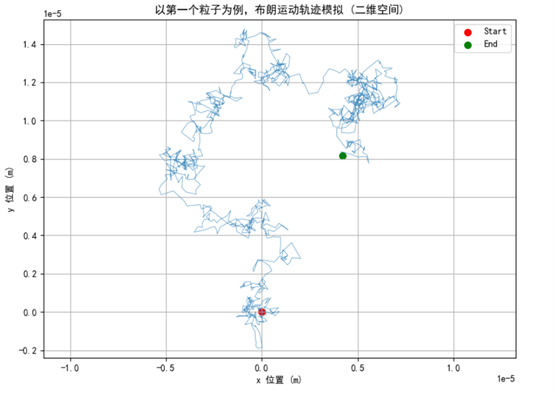
\includegraphics[width=0.9\textwidth]{trajectory.png}
  \caption{半径 $0.5~\mu$m 粒子的布朗运动轨迹示意}
  \label{fig:trajectory}
\end{figure}

对于多个半径 $0.5~\mu\text{m}$ 的粒子,在 $20^\circ$C 水溶液中做布朗运动时,其总 MSD 与时间满足:
\begin{align}
  \text{MSD}(t) &= 2Dt \quad &\text{(一维)} \\
  \text{MSD}(t) &= 4Dt \quad &\text{(二维)}
\end{align}

我们主要探究粒子在一维方向的运动特性。以其中 3 个粒子为例,其一维方向的位移随时间变化如图所示:

\begin{figure}[htbp]
  \centering
  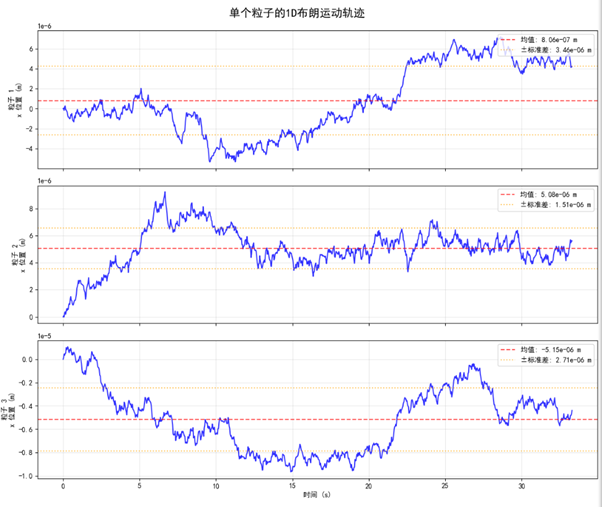
\includegraphics[width=0.9\textwidth]{displacement.png}
  \caption{三颗粒子在一维方向的位移随时间变化}
  \label{fig:displacement}
\end{figure}

\subsection{噪声对布朗运动的影响}

若在溶液环境中引入白噪声电场力,其作用可通过附加一项随机力 $\xi(t)$ 表示。对于直径 $0.5~\mu\text{m}$ 的粒子,随机电场力振幅 $\sigma$ 的定义为
\begin{equation}
  \sigma = q \frac{V_0}{d},
\end{equation}
其中,$q$ 为粒子所带电荷量,$V_0$ 为电极两端所加电压,$d$ 为电极间距。实验中,$\sigma$ 的数量级约为 $10^{-14}$,$d = 0.02~\text{m}$,$q \approx 10^{-16}$,因此 $V_0$ 设置在 $1$--$10~\text{V}$ 范围内。

在该条件下,粒子的有效温度会升高,但其 $x$ 方向位移依旧表现出一维随机布朗运动的性质。
\begin{figure}[htbp]
  \centering
  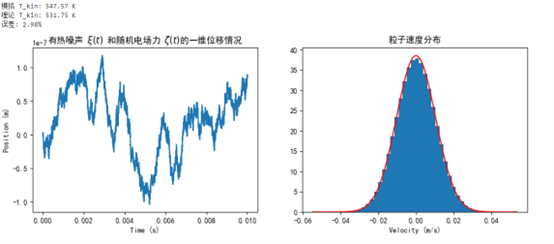
\includegraphics[width=0.9\textwidth]{一维位移.png}
  \caption{一维情况下的粒子}
  \label{fig:一维位移}
\end{figure}

\section{朗之万方程数值模拟与等效温度}

布朗运动在一维情况下可由朗之万方程描述:
\begin{equation}
  m \frac{dv}{dt} = -\gamma v + \xi(t) + \zeta(t),
\end{equation}
其中,$\gamma$ 为摩擦系数,$\xi(t)$ 表示热噪声,$\zeta(t)$ 表示外加电噪声。根据能量均分定理,定义等效动能温度为
\begin{equation}
  T_{\text{eff}} = \frac{m \langle v^2 \rangle}{k_B},
\end{equation}
其中 $k_B$ 为玻尔兹曼常数,$m$ 为粒子质量,$\langle v^2 \rangle$ 为速度方差。

\section{不同 $\sigma$ 下的扩散系数拟合}

当引入噪声时,扩散系数随 $\sigma$ 的变化关系可表示为
\begin{equation}
  D = D_0 + k\sigma^2,
\end{equation}
其中 $D_0$ 为无外加噪声时的扩散系数,$k$ 为拟合系数。因此,$D$ 与 $\sigma$ 呈二次曲线关系。

\begin{figure}[htbp]
  \centering
  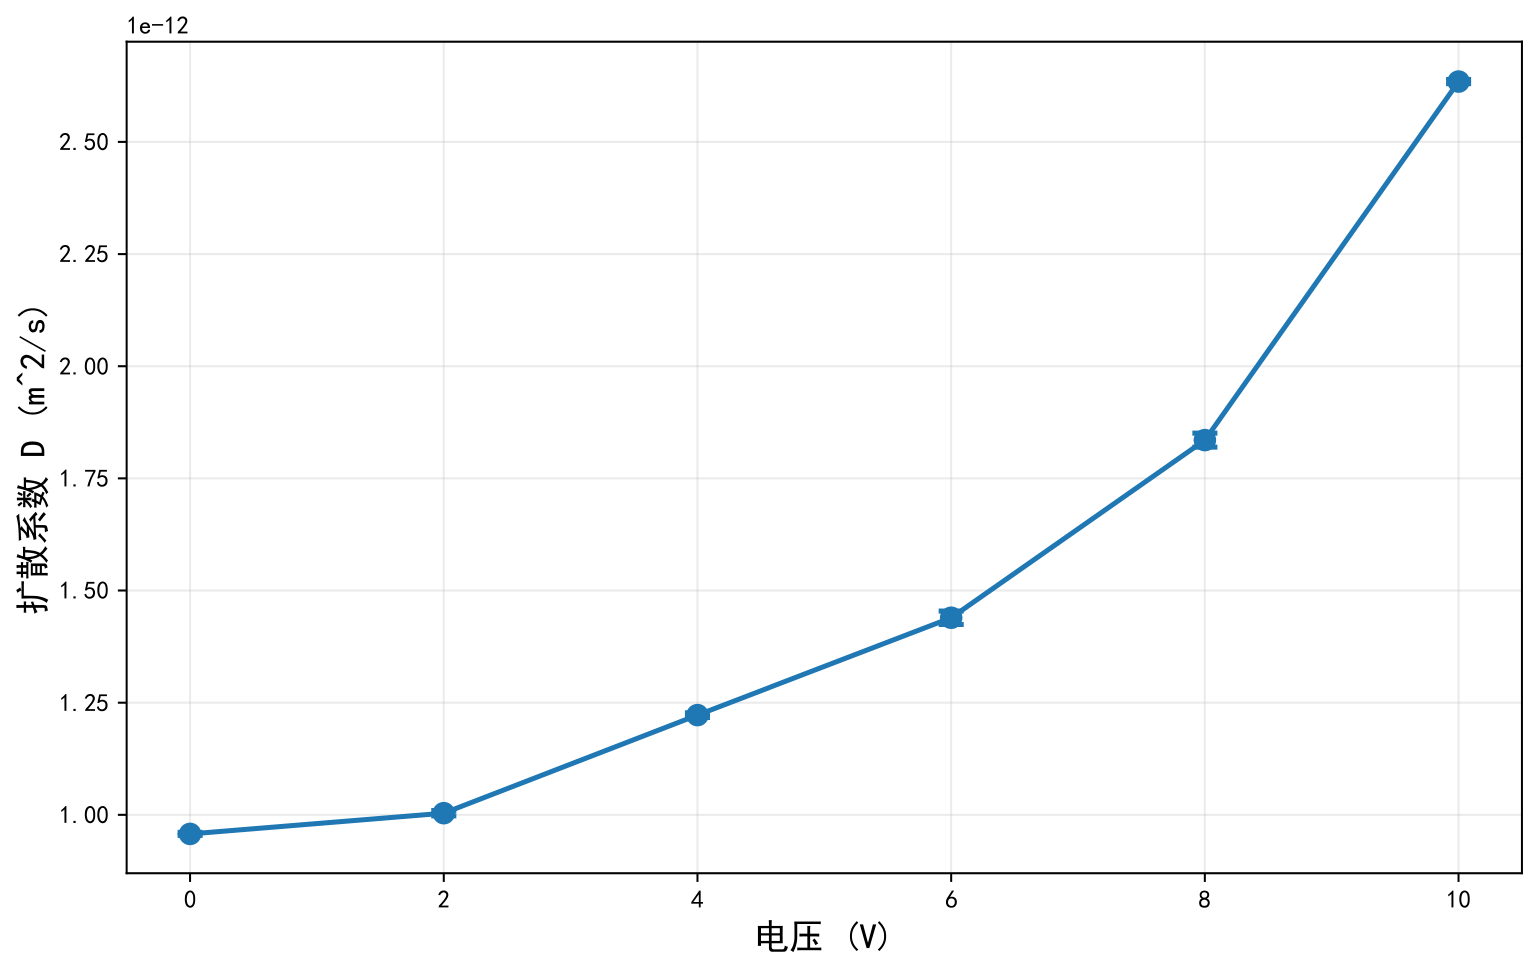
\includegraphics[width=0.9\textwidth]{fit.png}
  \caption{不同噪声强度下扩散系数 $D$ 的拟合结果}
  \label{fig:fit}
\end{figure}


\chapter{装置设计}
\section{实验仪器与设计}
由于水平放置的样品容易受到重力作用,悬浮粒子会逐渐沉降至样品底部,进而受到附加阻力的影响,导致微球的布朗运动减弱,
不利于作为理想的实验对象\cite{einstein1905,dhont1996brownian}。\par
因此,本实验采用垂直放置样品的设计,以最大程度减小重力对粒子运动的干扰。垂直放置不仅能够更好地匹配显微镜的光学路径,
从而提升成像质量与分辨率,还能更准确地捕捉布朗粒子的运动轨迹。此外,该设计也便于电极的插入与固定,为后续加载噪声信号提供了实验条件。\par

在光源选择方面,本实验采用非相干光源作为照明。相比于相干光,非相干光源具有较宽的光谱范围和较低的相干性,可有效抑制干涉和衍射效应,
从而提升成像的均匀性与清晰度,更适合布朗粒子的观测需求\cite{goodman,mandel1995optical}。\par

对于噪声的引入,本实验利用信号发生器产生可控的电噪声信号。
通过调节其输出频率与幅度,可精确控制噪声特性,以适应不同实验条件\cite{horowitz1989art,schreiber1999electrical}。

实验所用主要仪器如下:
分辨率板为 USAF 1951;100$\times$ 物镜(SOPTOP,NA = 0.80,工作距离 2~mm,有限远校正);
CCD 为海康机器人,分辨率 5472$\times$3648,像素间距 2~$\mu$m,20~fps;信号发生器型号为固纬 AFG-2225。
\begin{figure}[htbp]
    \centering
    % 每行 4 张
    \begin{subfigure}{0.22\textwidth}
        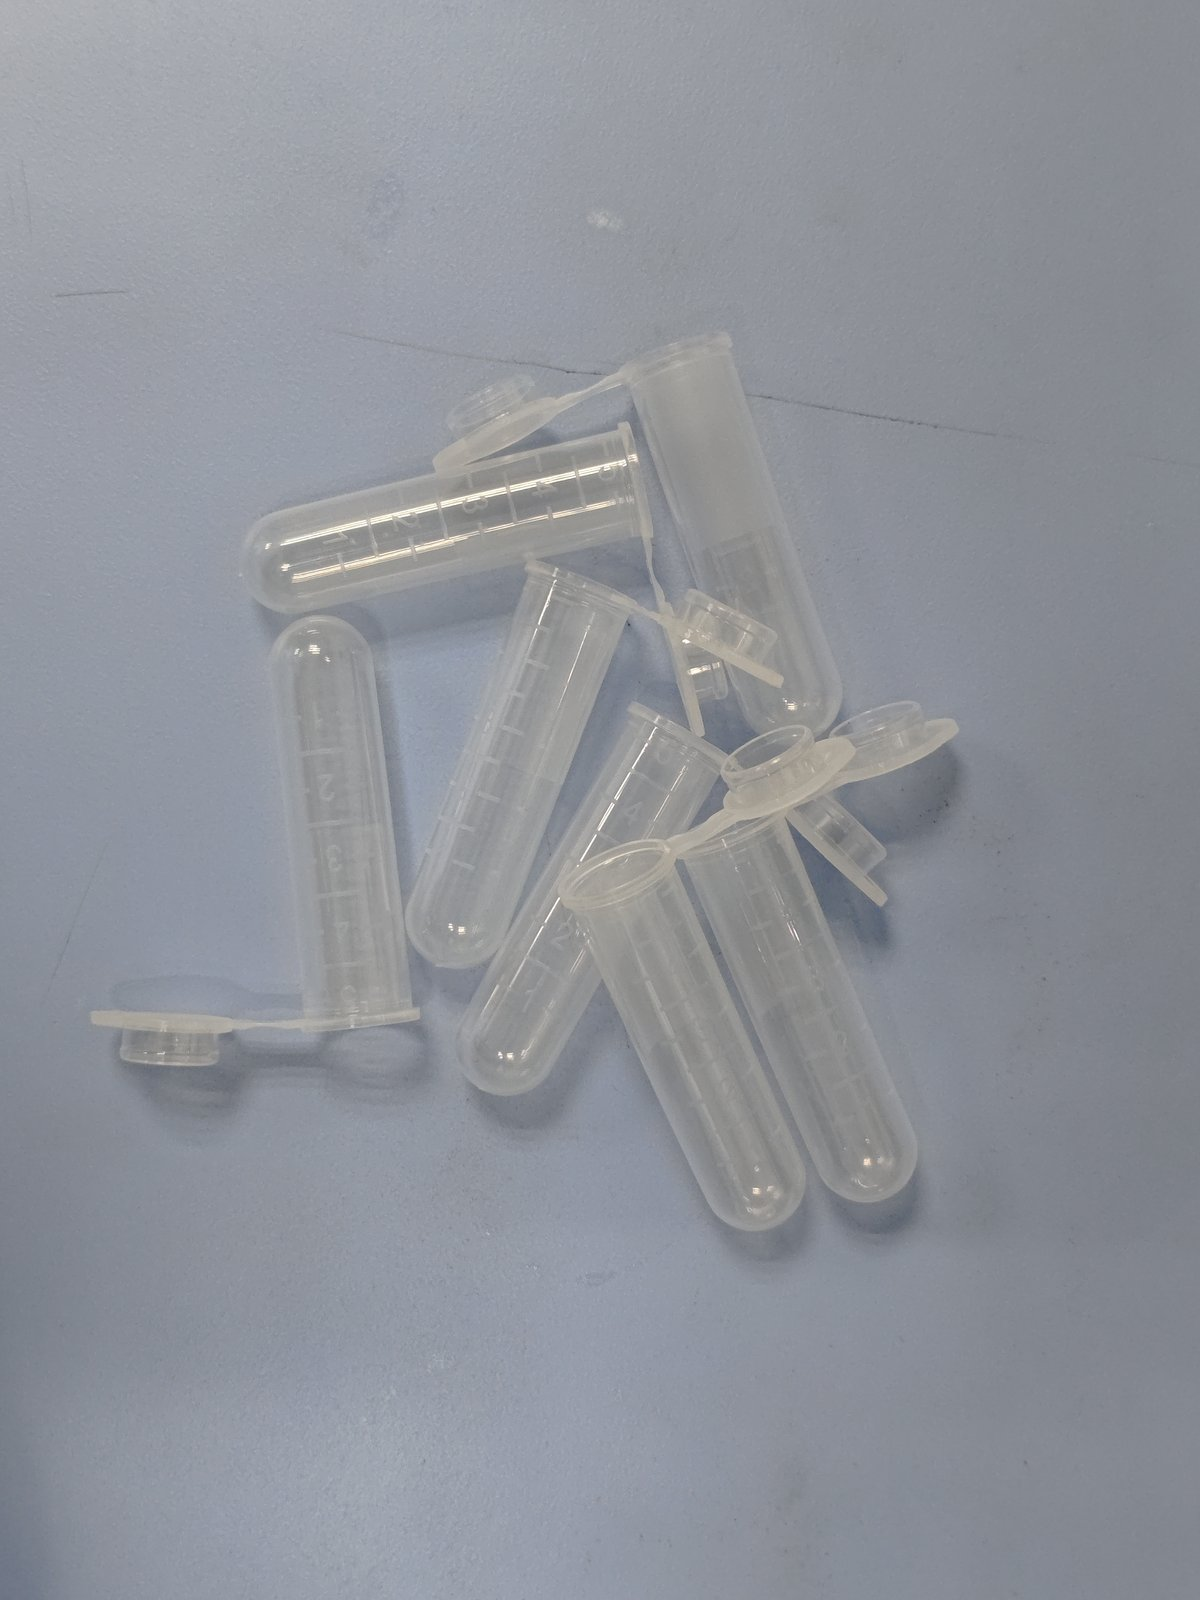
\includegraphics[width=\linewidth]{5.0ml微量离心管.jpg}
        \caption{5.0ml微量离心管}
    \end{subfigure}
    \begin{subfigure}{0.22\textwidth}
        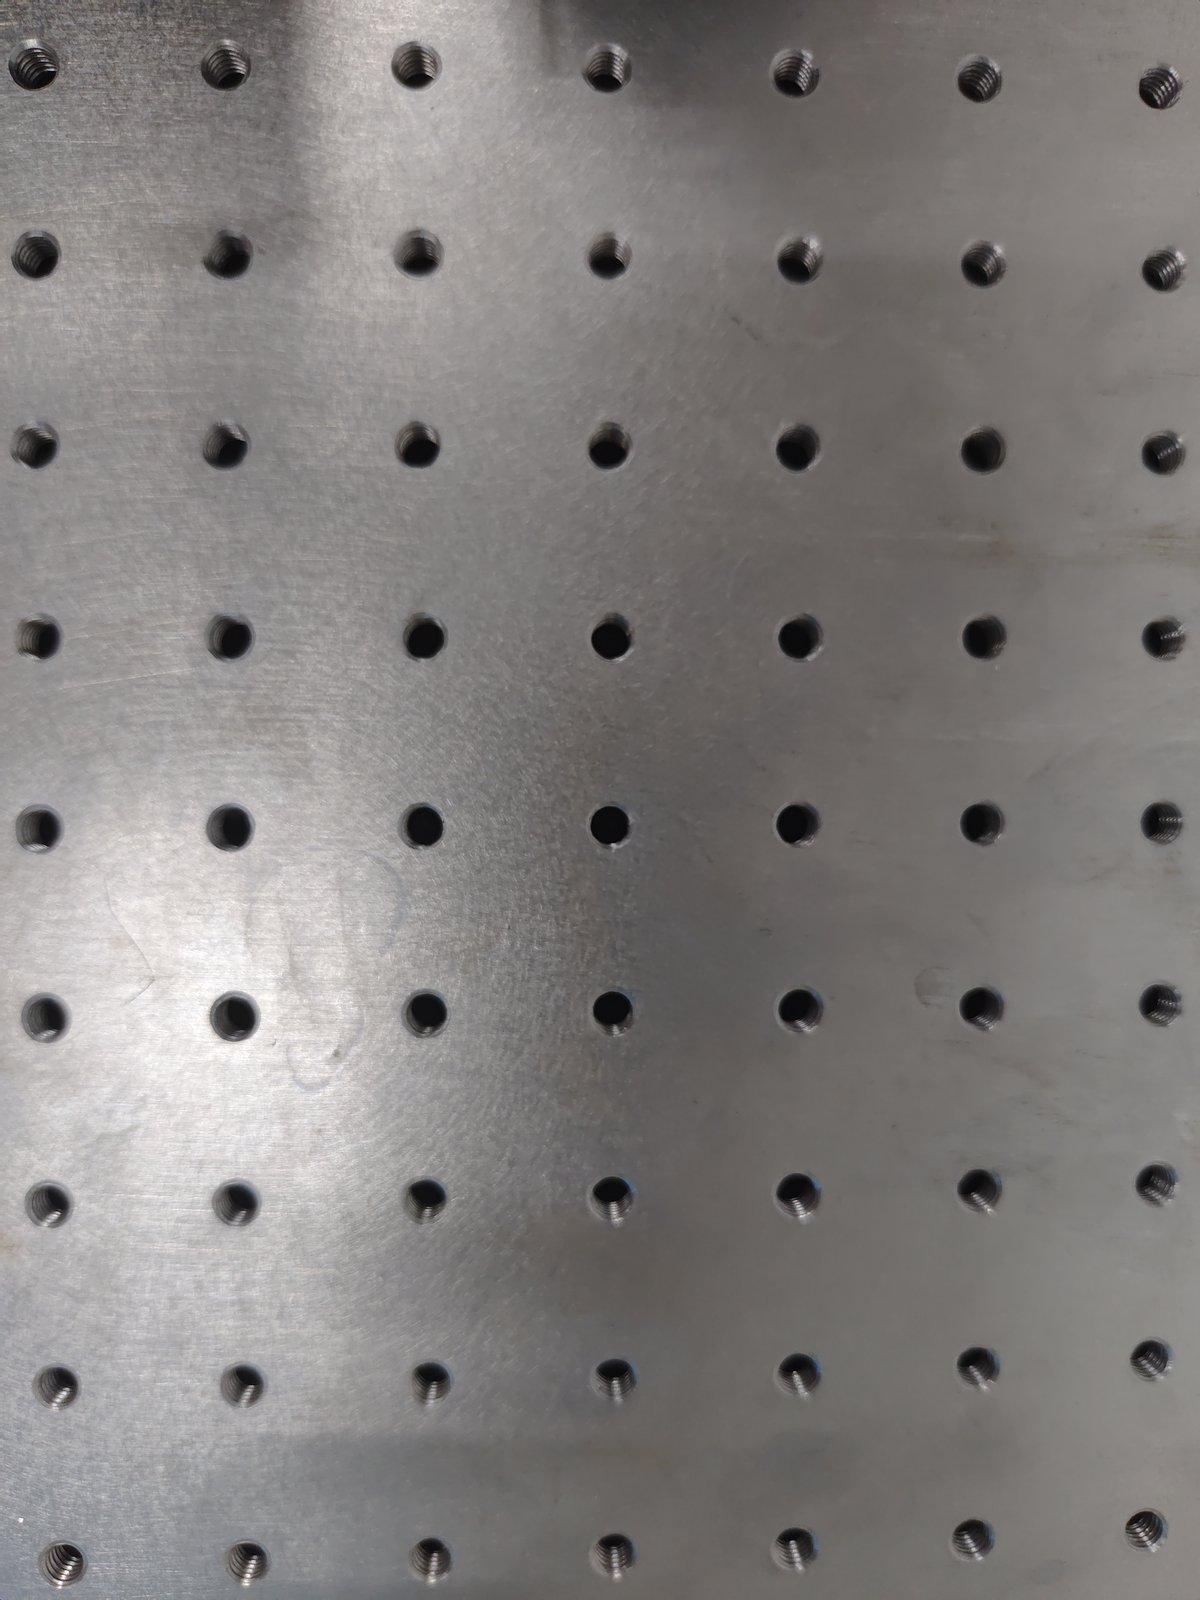
\includegraphics[width=\linewidth]{光学平台.jpg}
        \caption{光学平台}
    \end{subfigure}
    \begin{subfigure}{0.22\textwidth}
        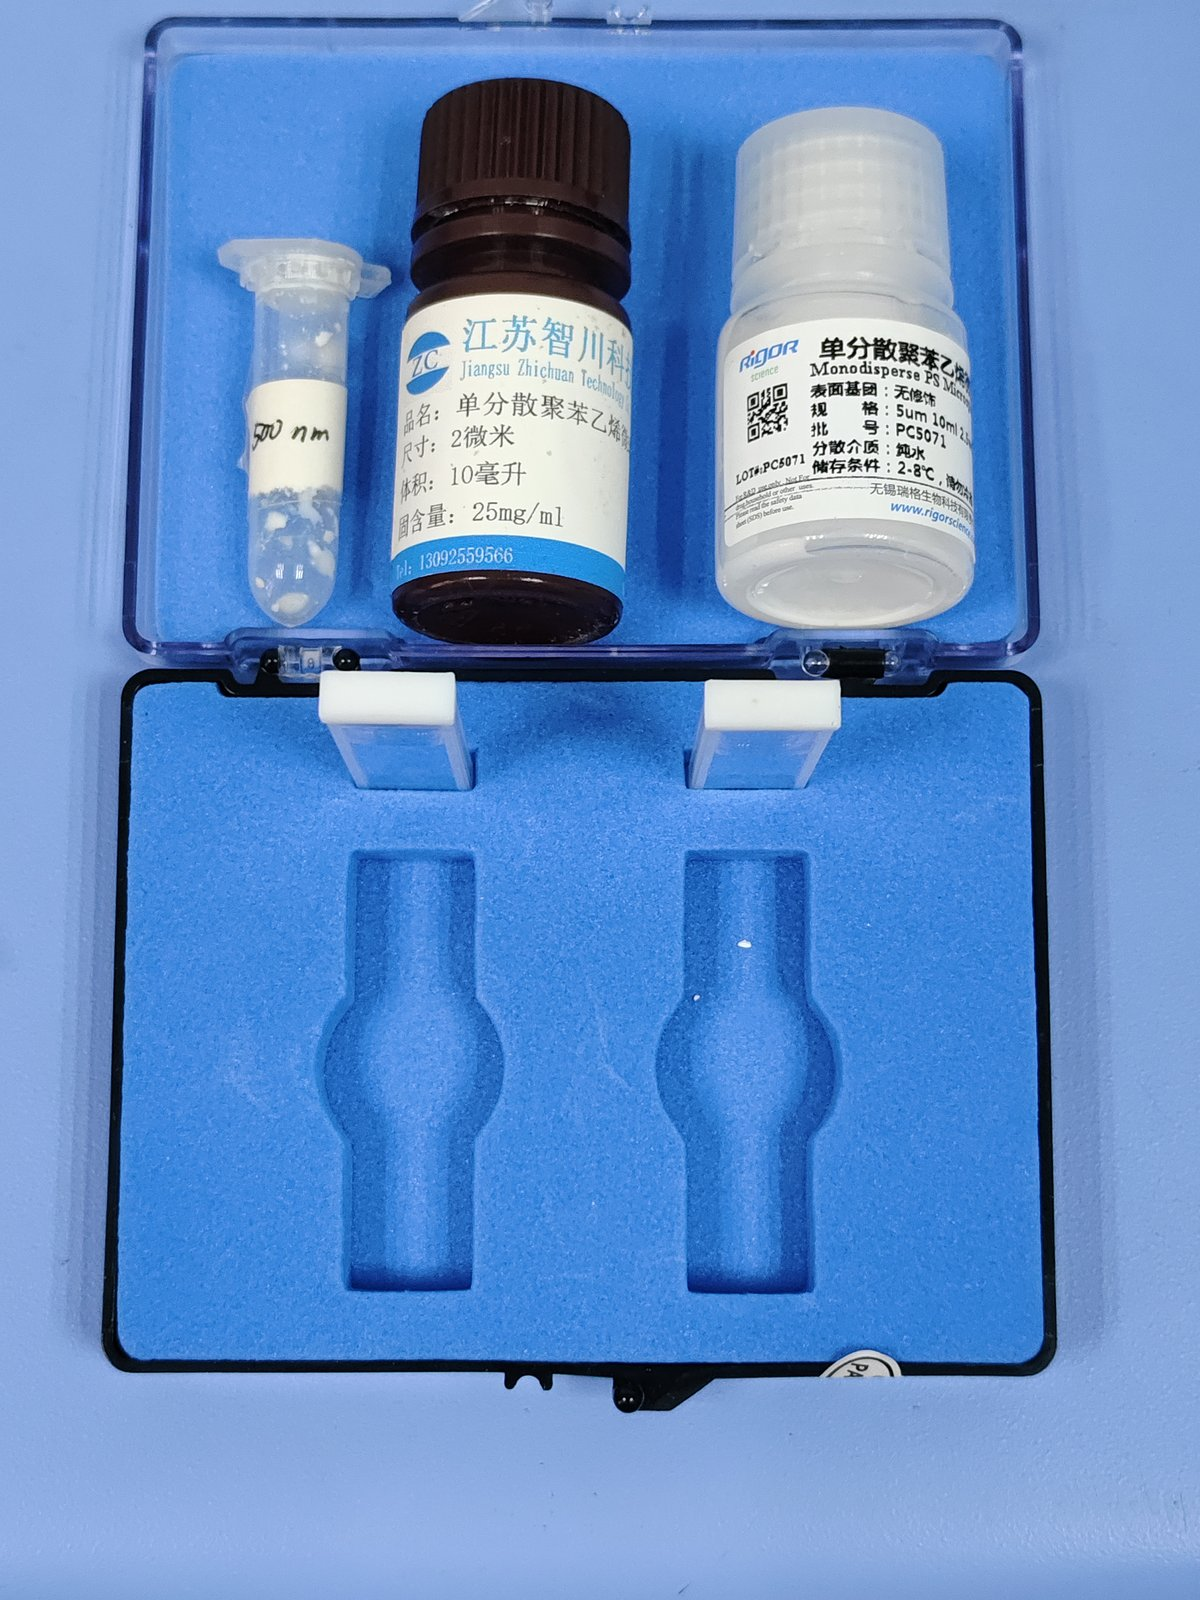
\includegraphics[width=\linewidth]{比色皿.jpg}
        \caption{比色皿}
    \end{subfigure}
    \begin{subfigure}{0.22\textwidth}
        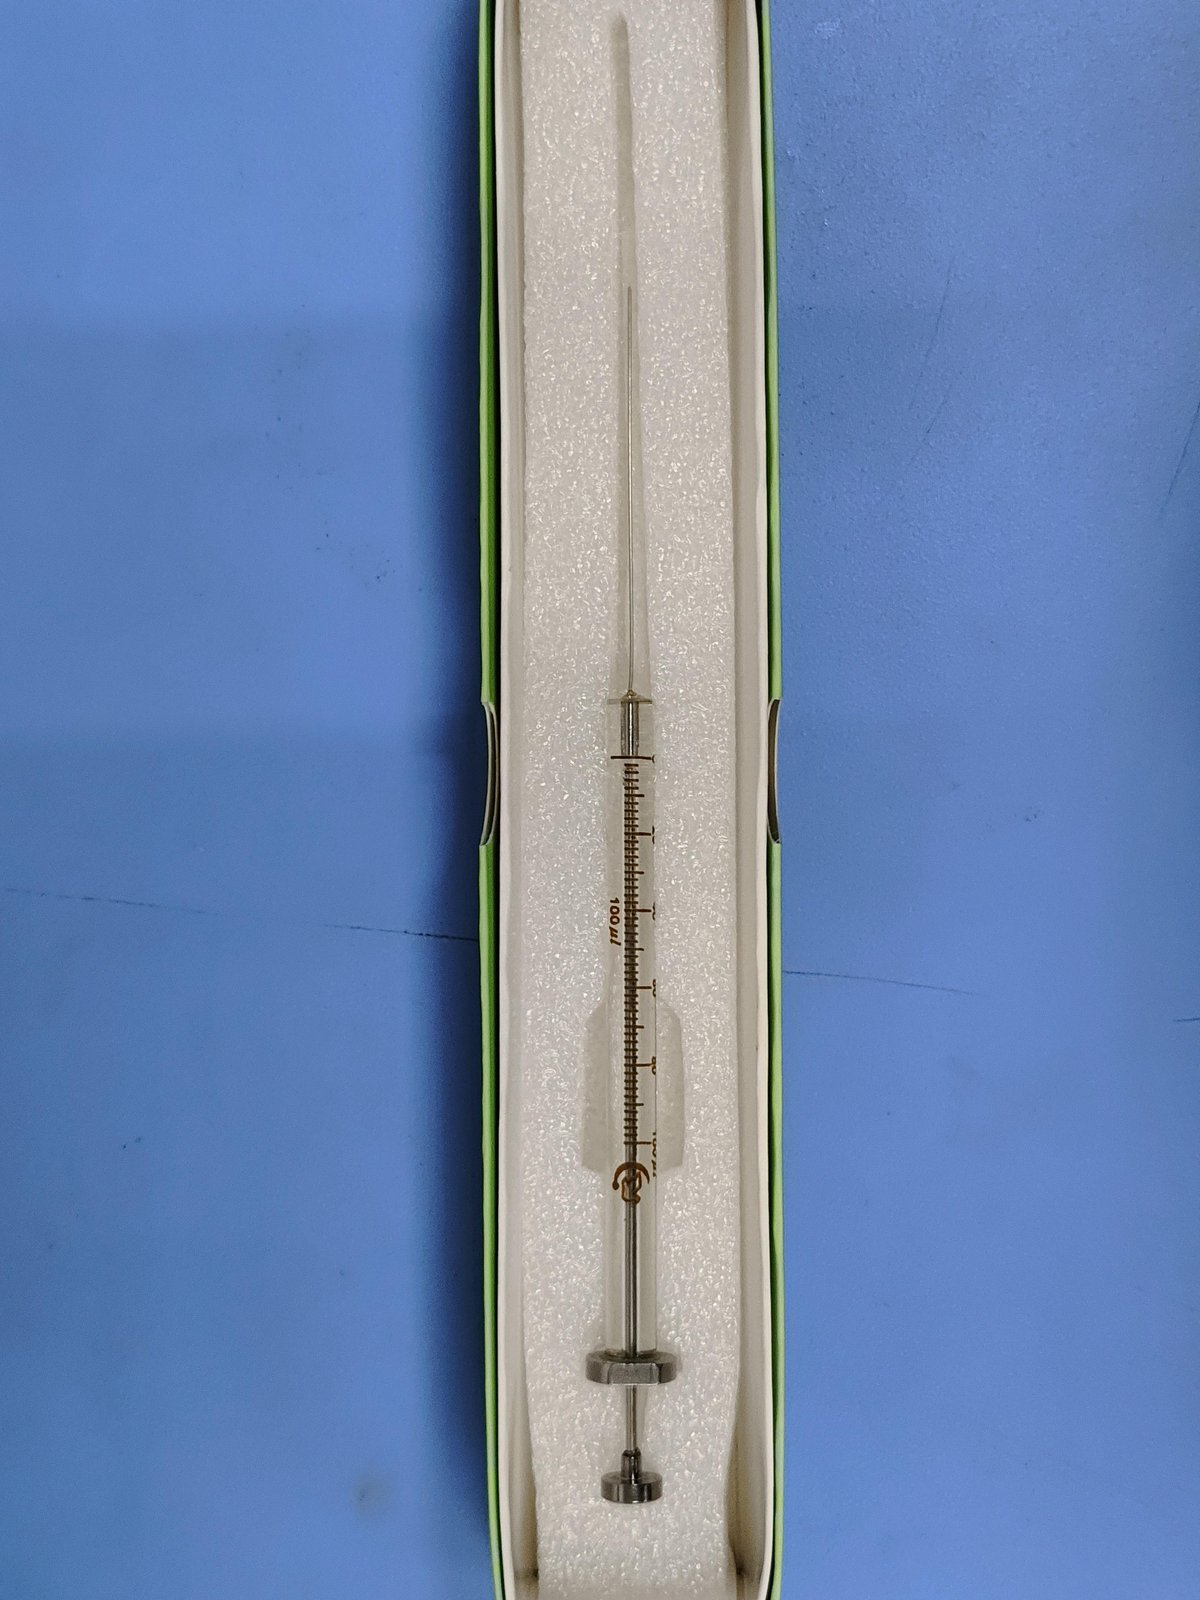
\includegraphics[width=\linewidth]{微量进样器.jpg}
        \caption{微量进样器}
    \end{subfigure}

    % 第二行
    \begin{subfigure}{0.22\textwidth}
        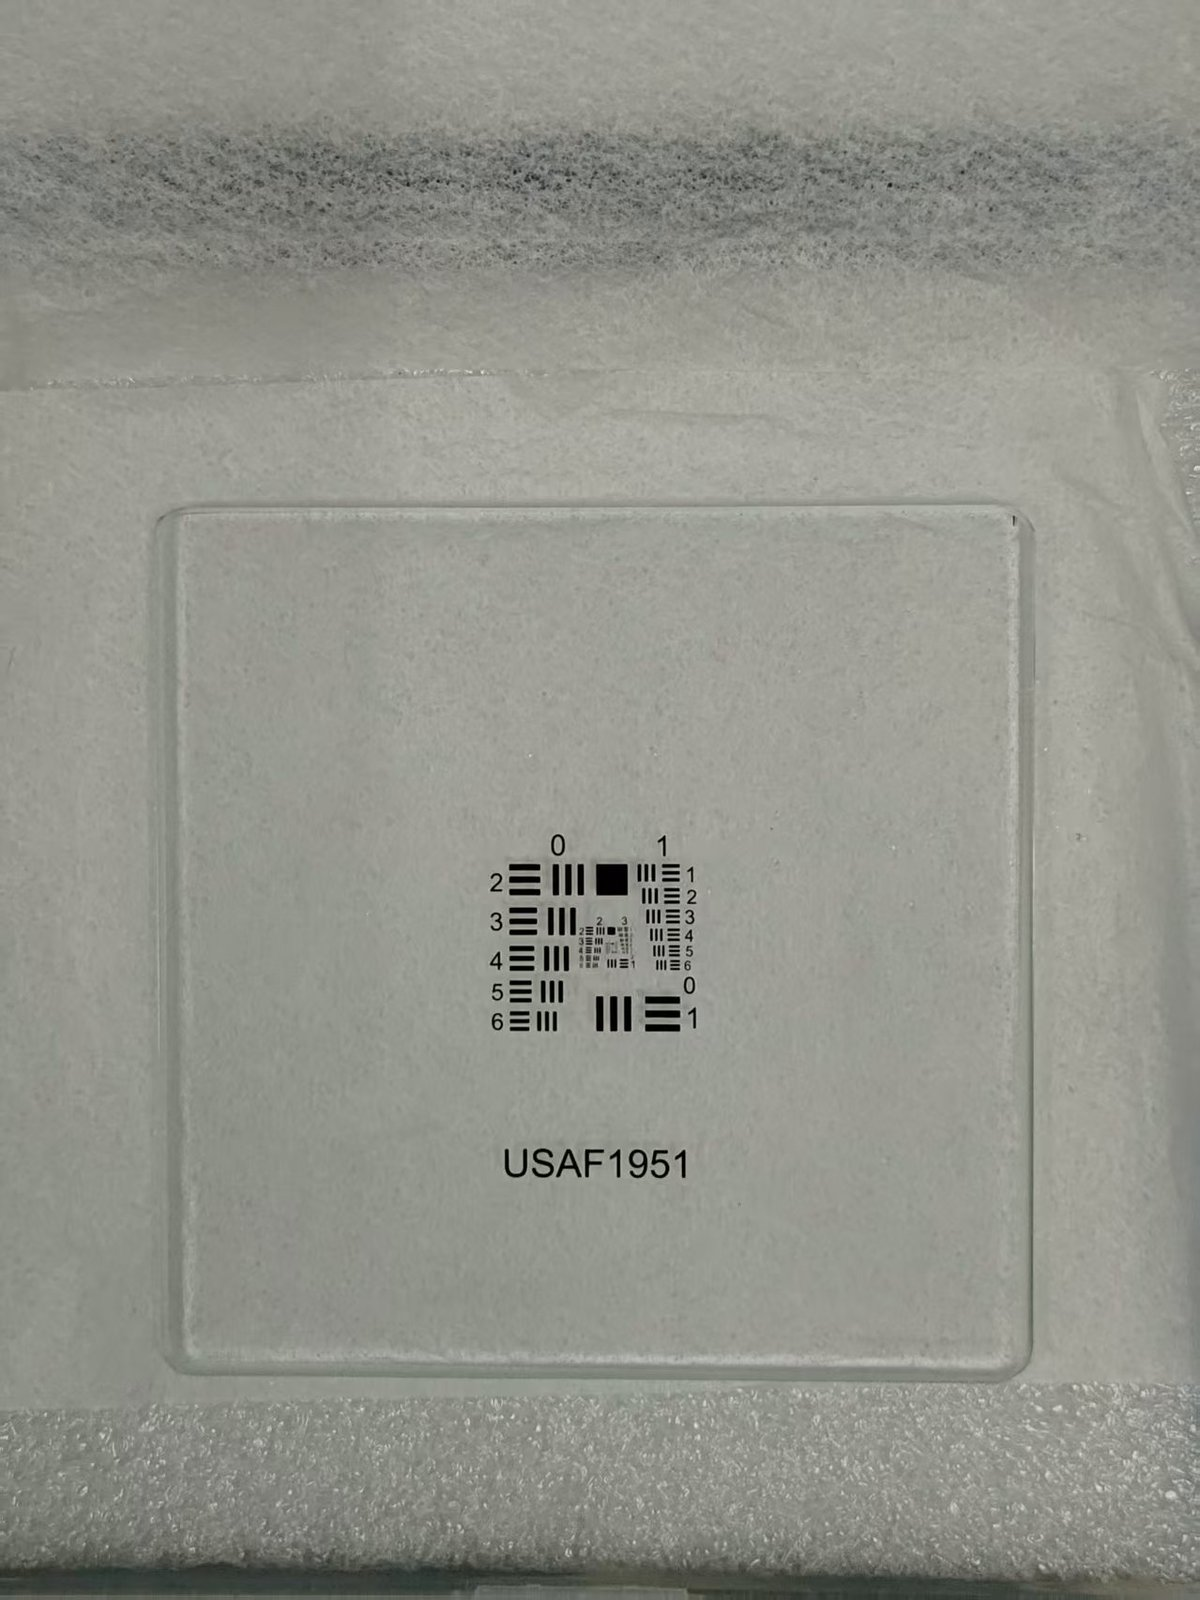
\includegraphics[width=\linewidth]{分辨率板.jpg}
        \caption{分辨率板}
    \end{subfigure}
    \begin{subfigure}{0.22\textwidth}
        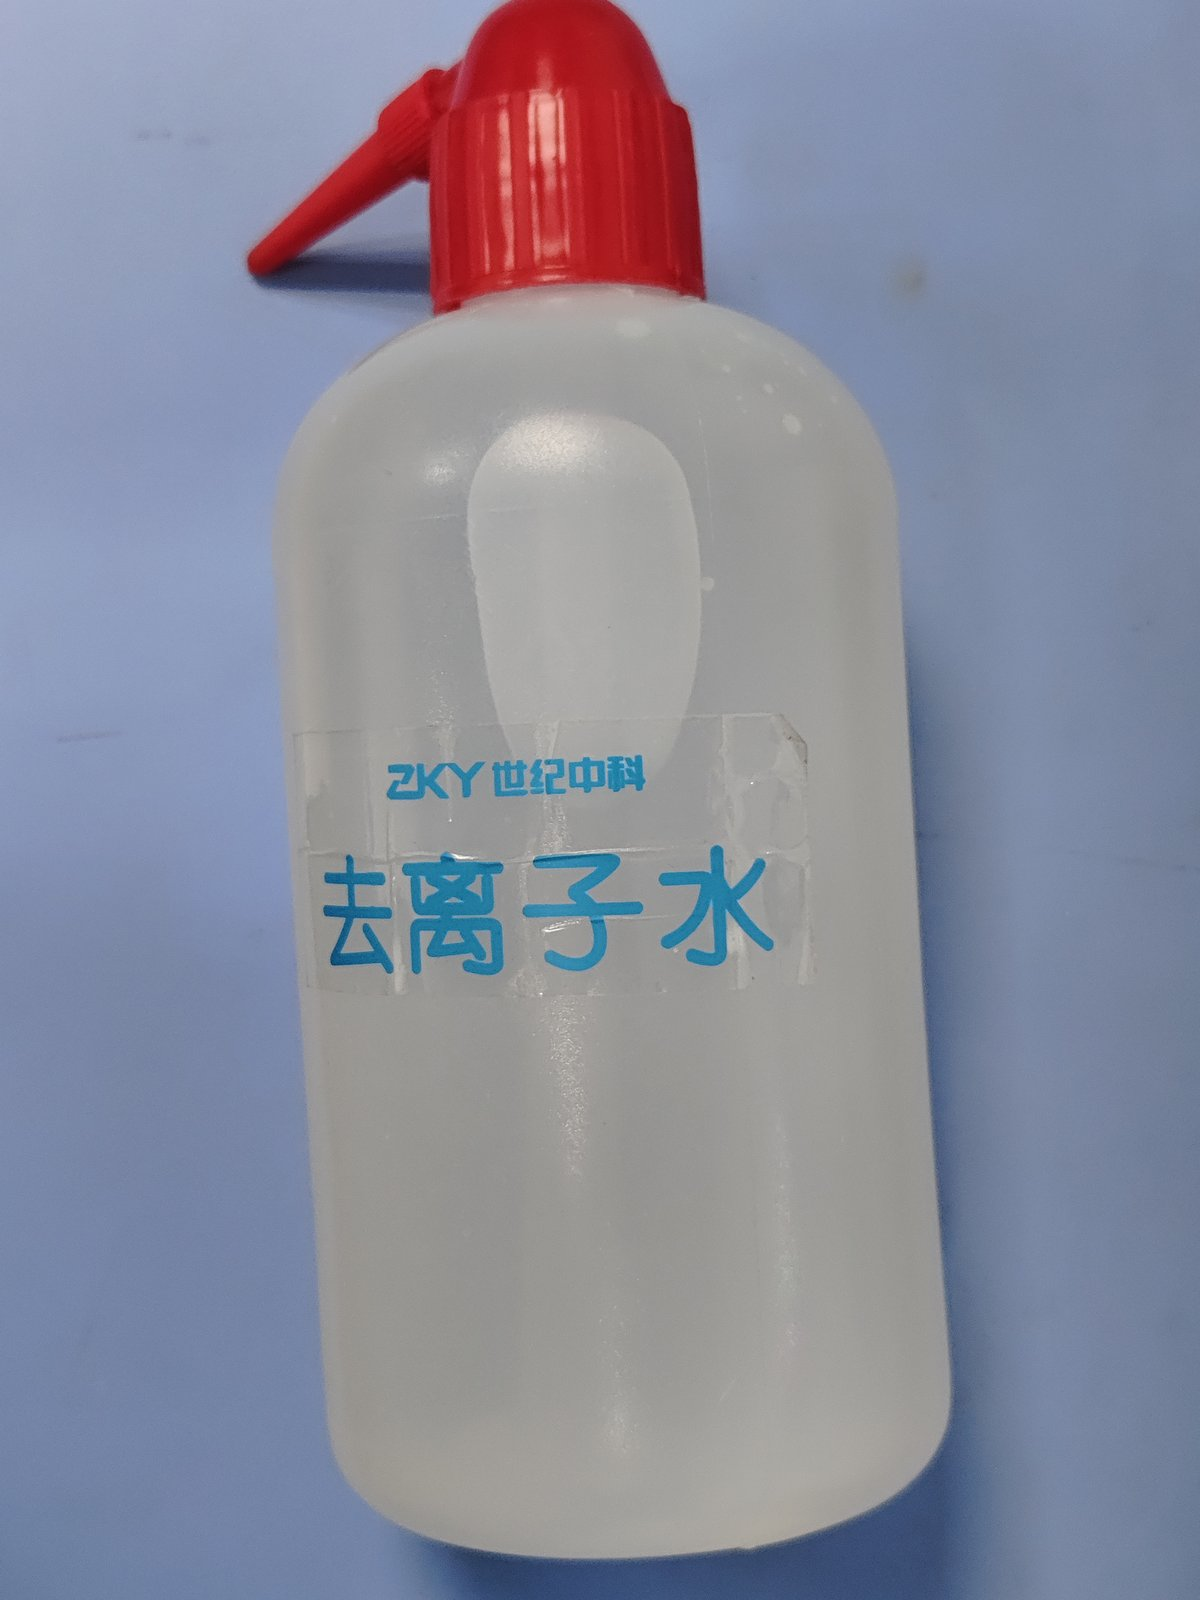
\includegraphics[width=\linewidth]{去离子水.jpg}
        \caption{去离子水}
    \end{subfigure}
    \begin{subfigure}{0.22\textwidth}
        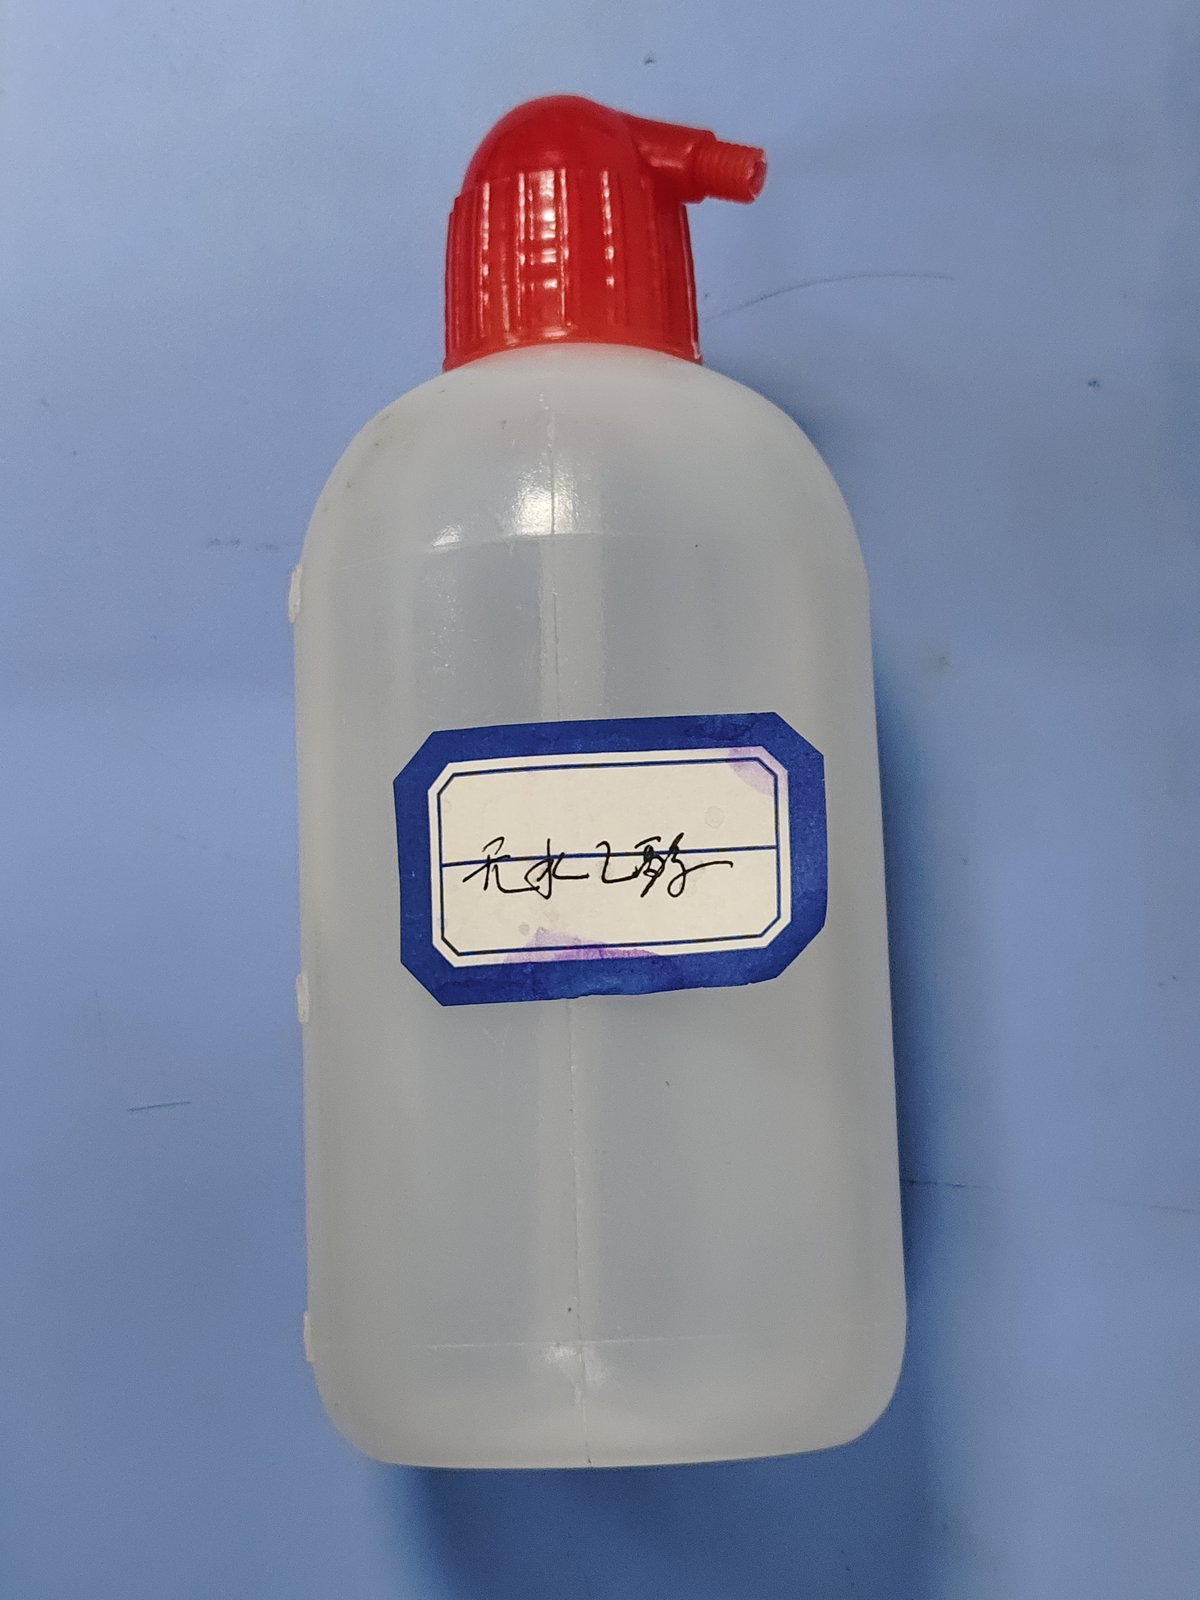
\includegraphics[width=\linewidth]{无水乙醇.jpg}
        \caption{无水乙醇}
    \end{subfigure}
    \begin{subfigure}{0.22\textwidth}
        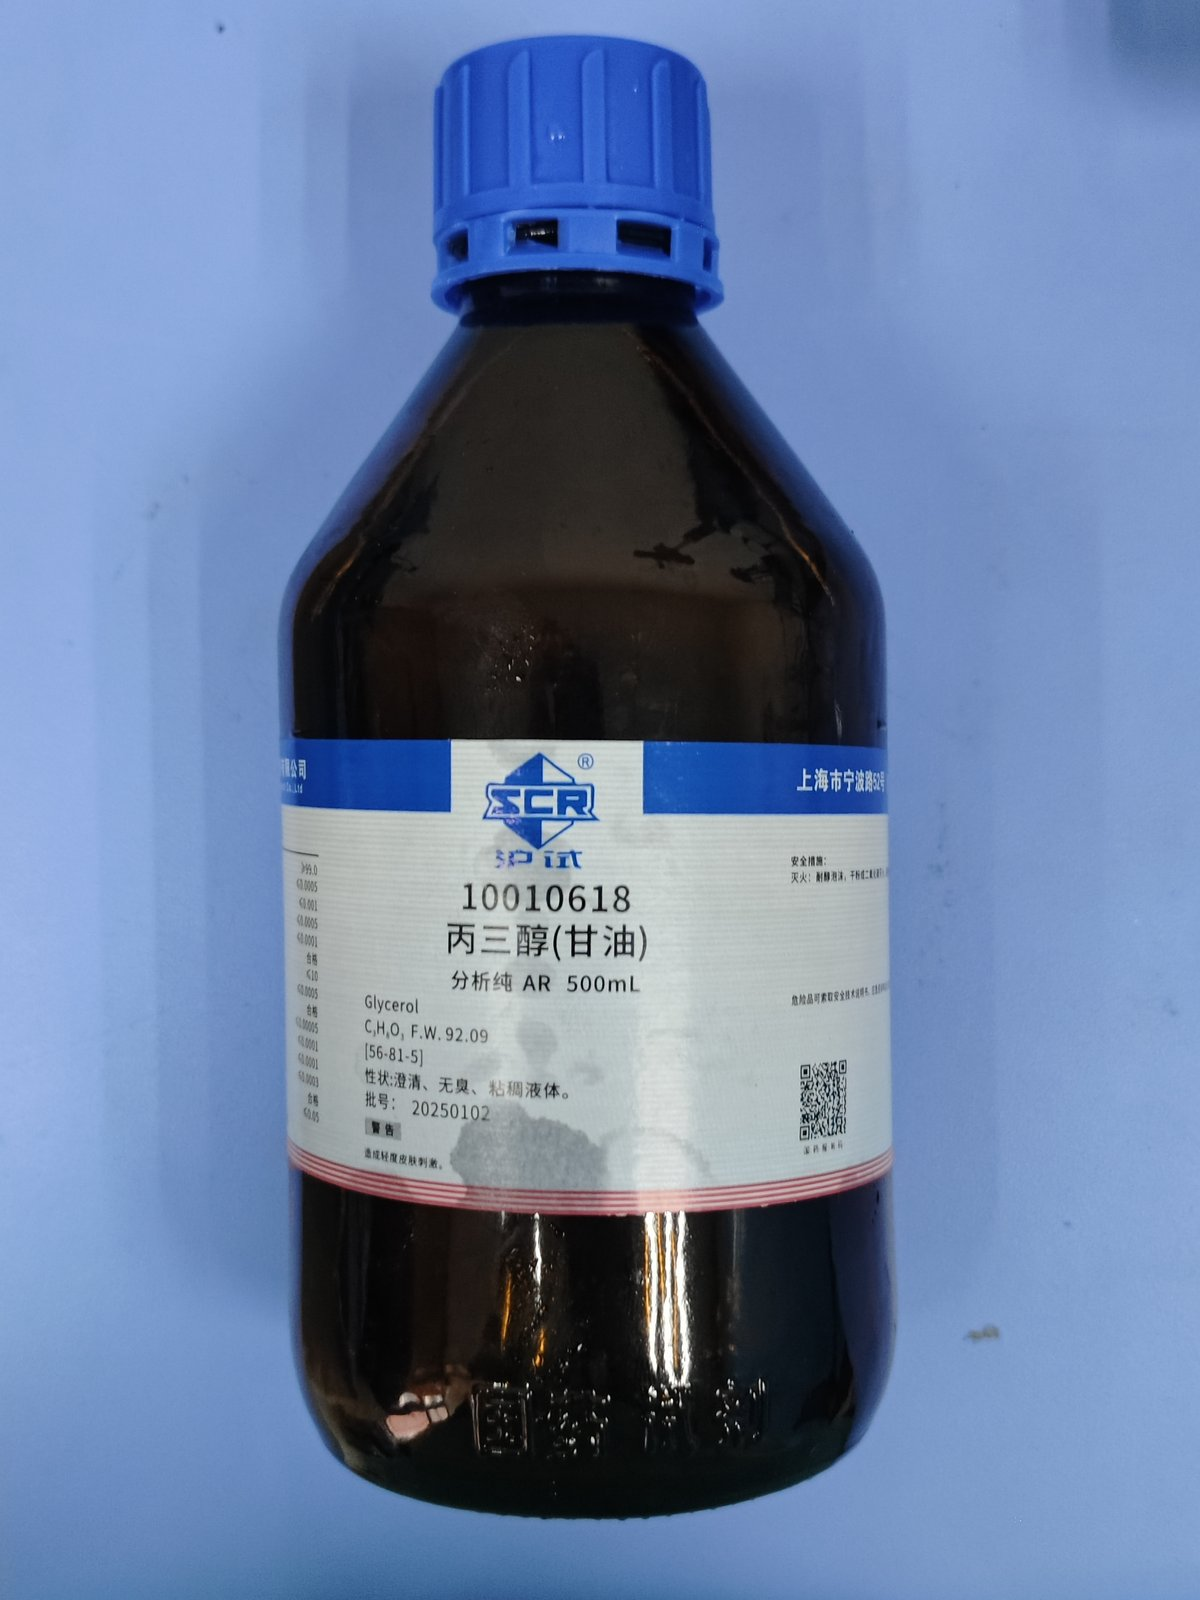
\includegraphics[width=\linewidth]{甘油.jpg}
        \caption{甘油}
    \end{subfigure}

    % 第三行
    \begin{subfigure}{0.22\textwidth}
        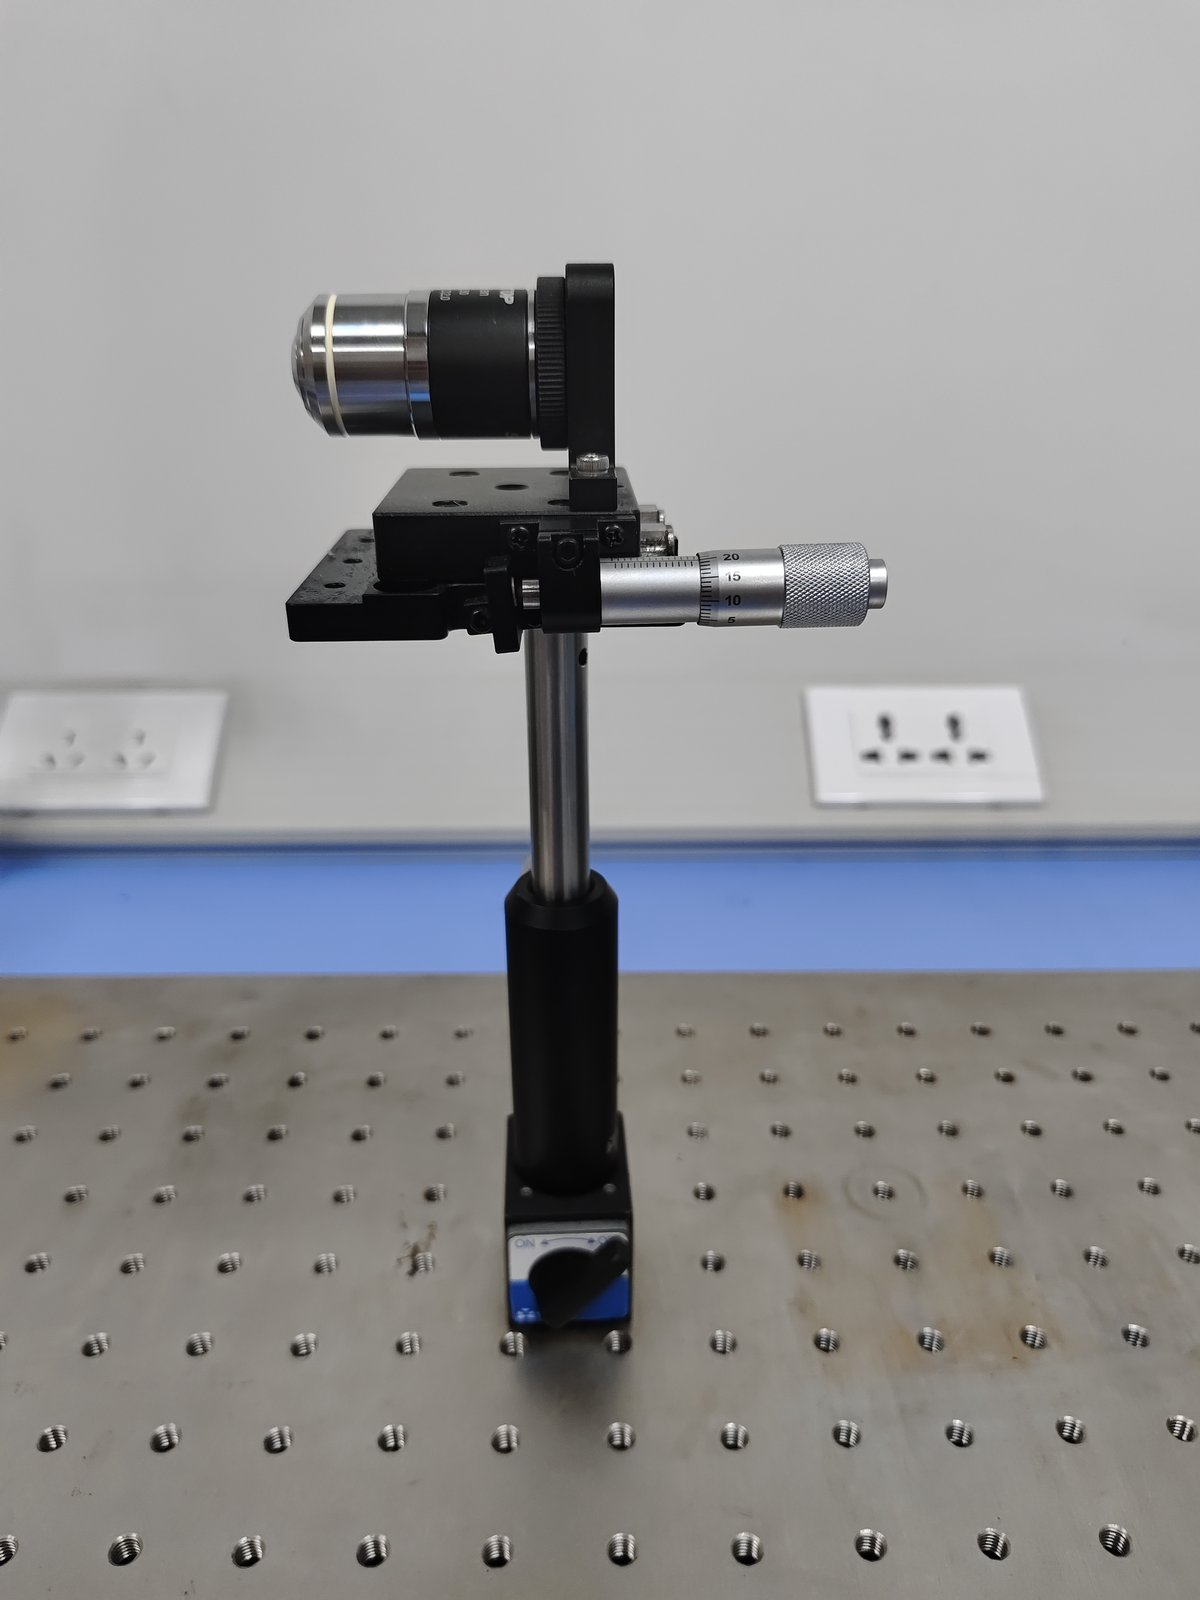
\includegraphics[width=\linewidth]{100x物镜.jpg}
        \caption{100x物镜}
    \end{subfigure}
    \begin{subfigure}{0.22\textwidth}
        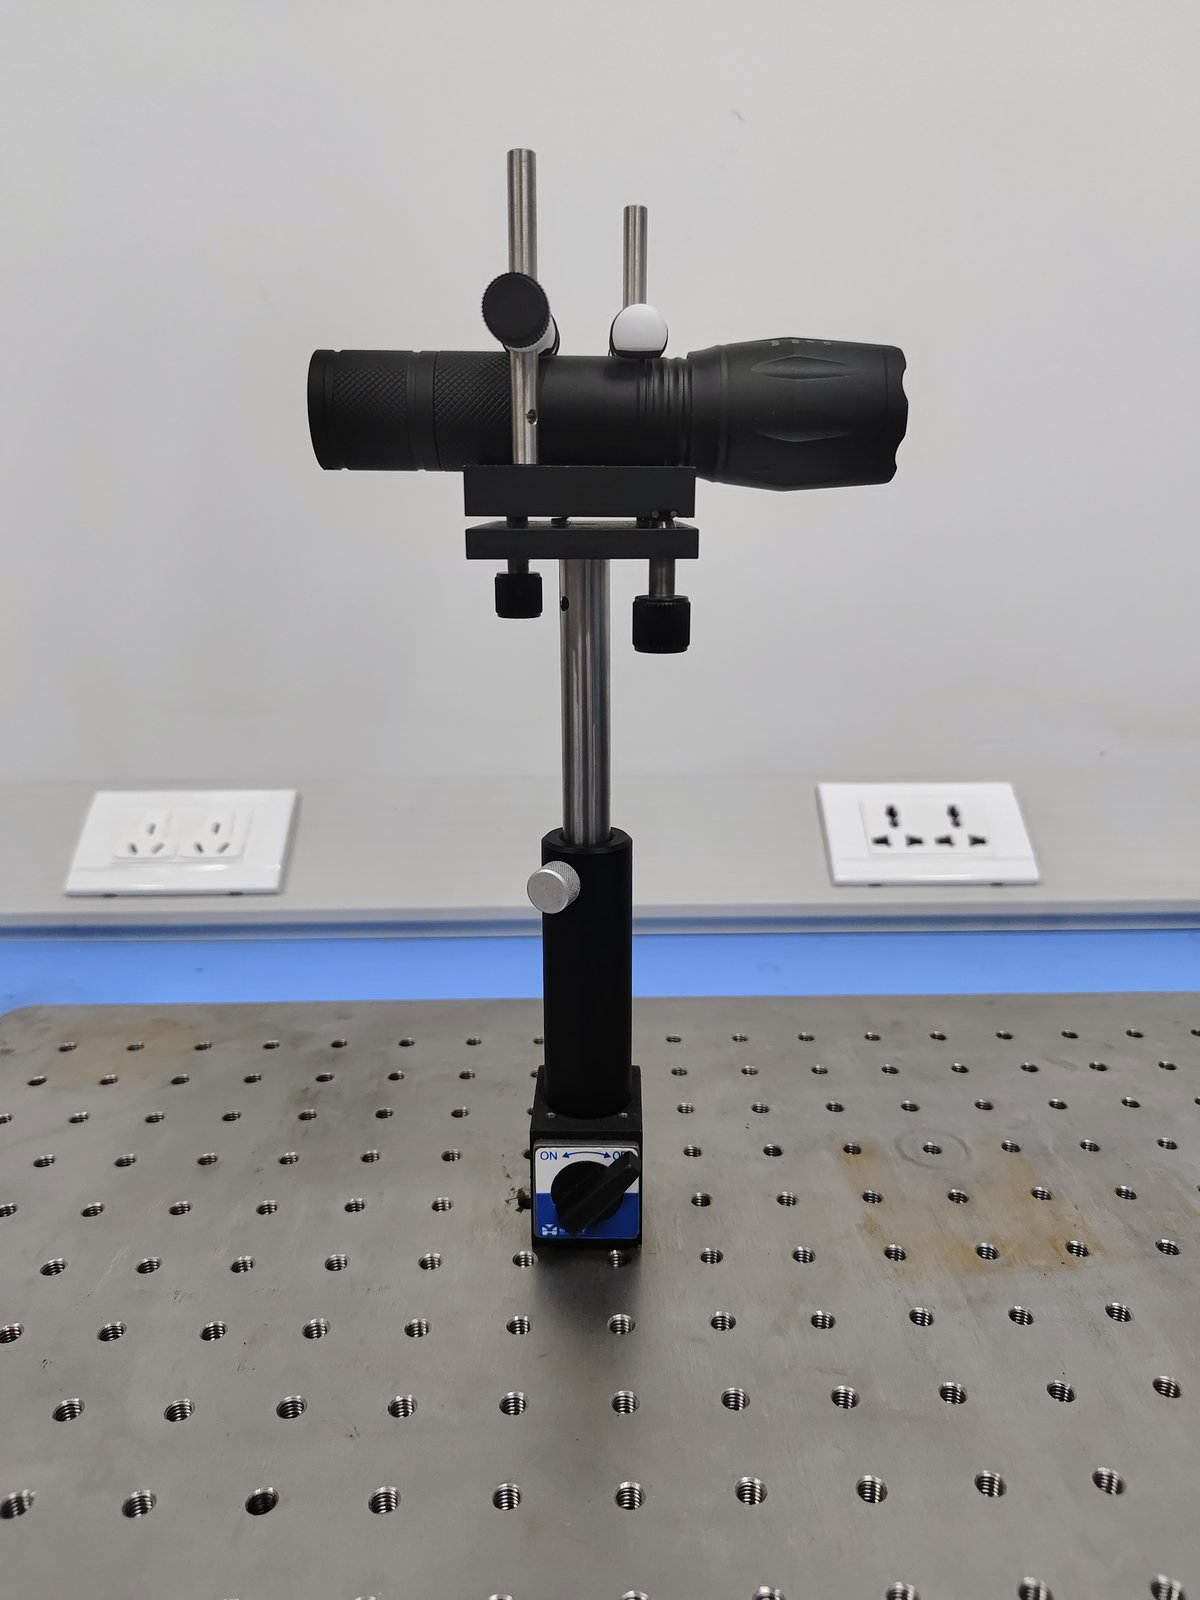
\includegraphics[width=\linewidth]{非相干光源.jpg}
        \caption{非相干光源}
    \end{subfigure}
    \begin{subfigure}{0.22\textwidth}
        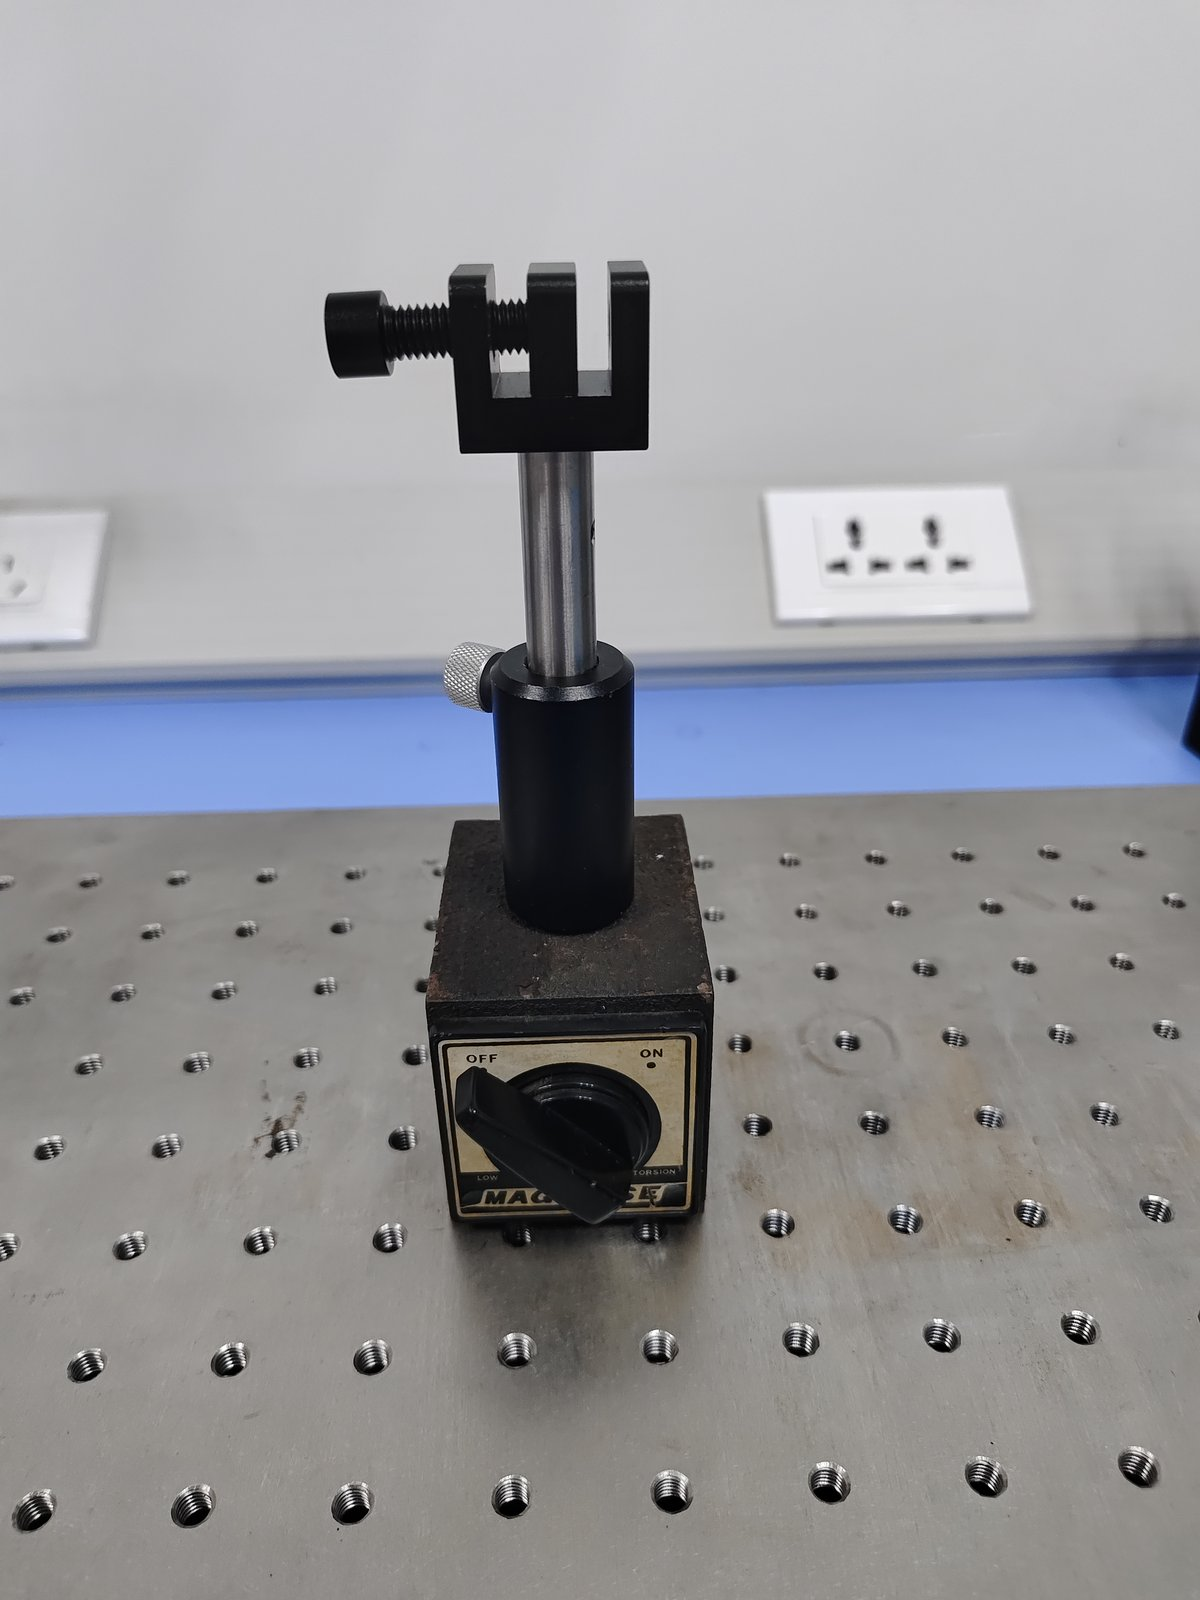
\includegraphics[width=\linewidth]{夹具1.jpg}
        \caption{夹具}
    \end{subfigure}
    \begin{subfigure}{0.22\textwidth}
        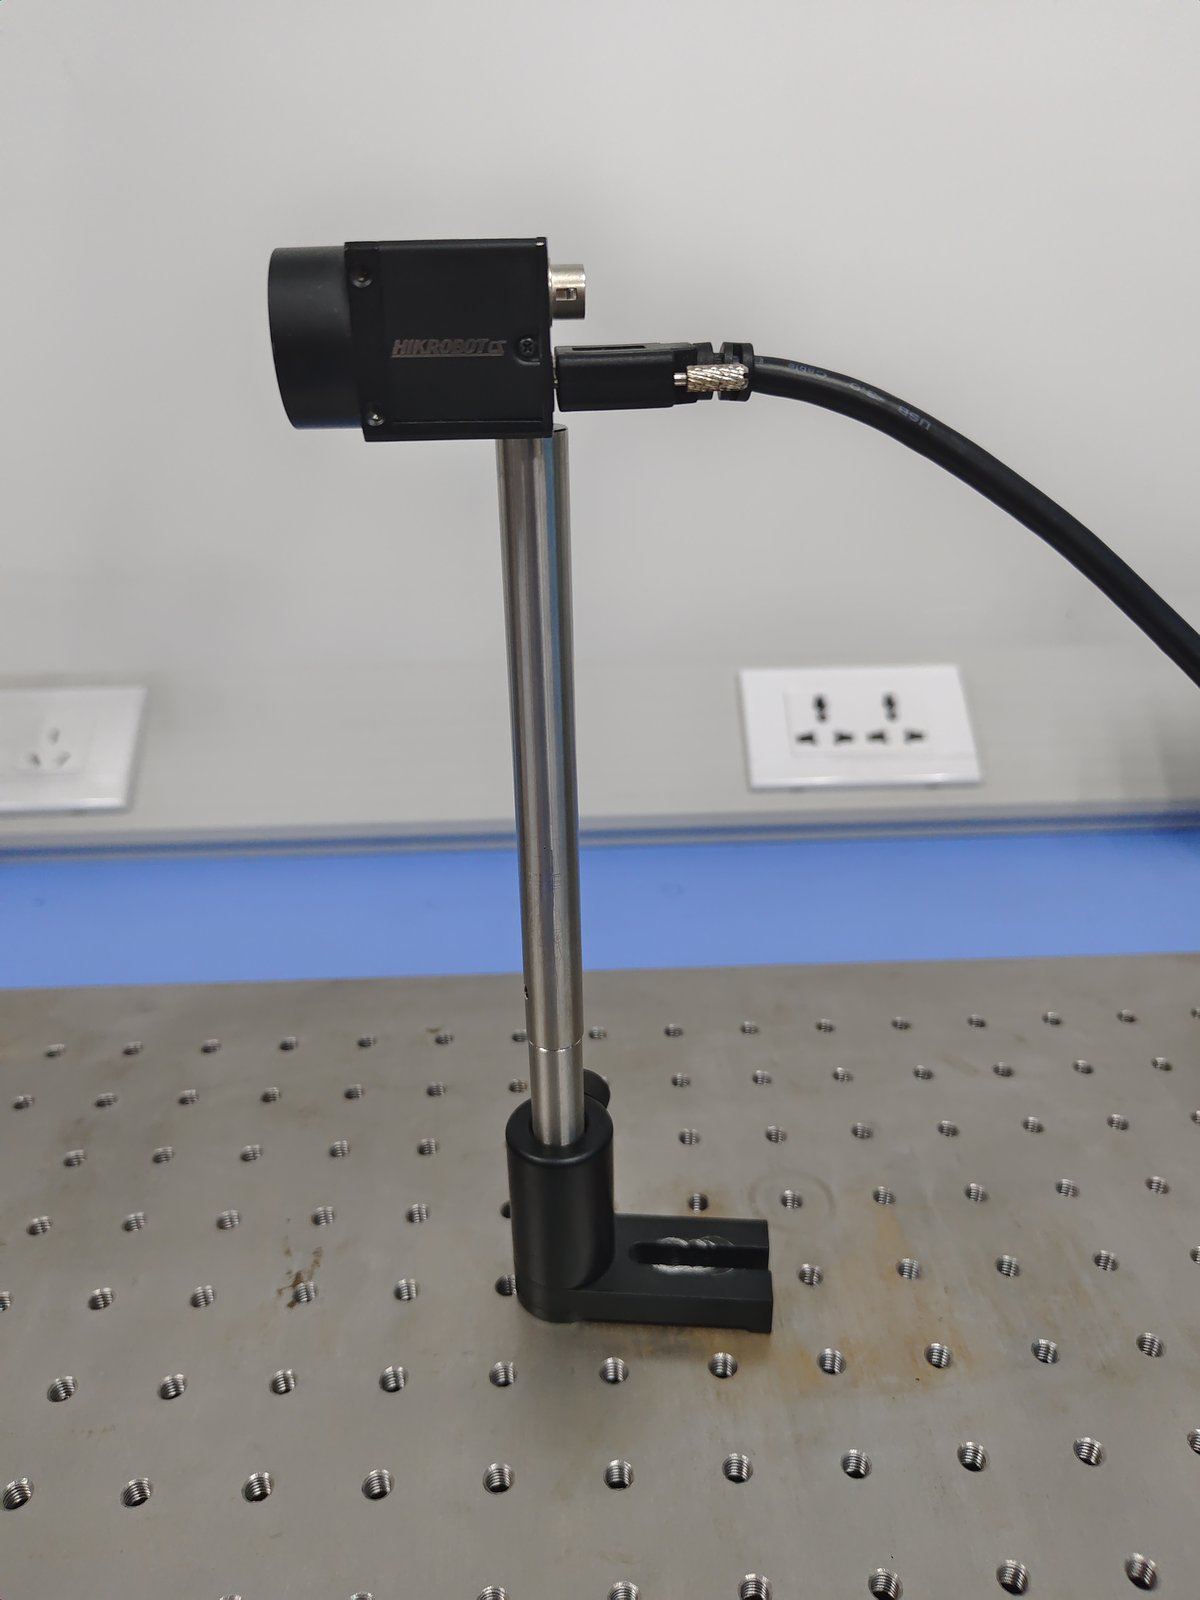
\includegraphics[width=\linewidth]{CCD.jpg}
        \caption{CCD}
    \end{subfigure}

    % 第四行
    \begin{subfigure}{0.22\textwidth}
        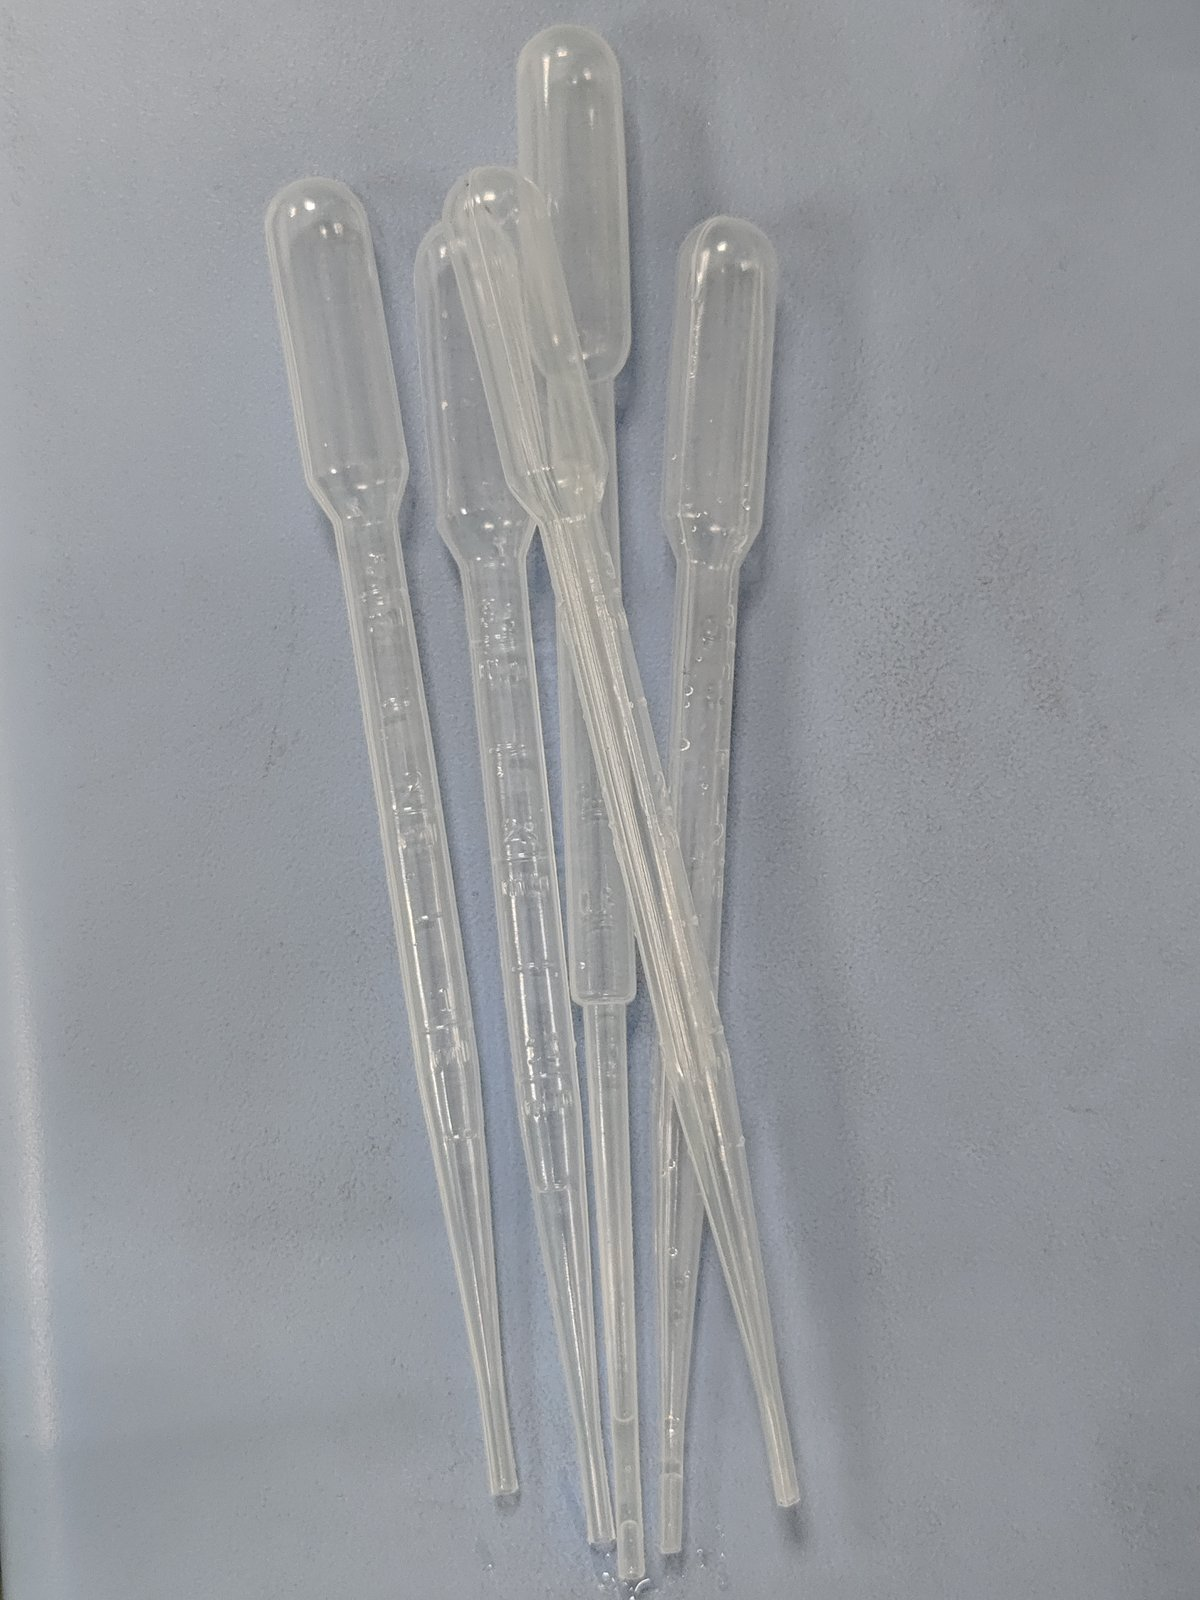
\includegraphics[width=\linewidth]{胶头滴管.jpg}
        \caption{胶头滴管}
    \end{subfigure}
    \begin{subfigure}{0.22\textwidth}
        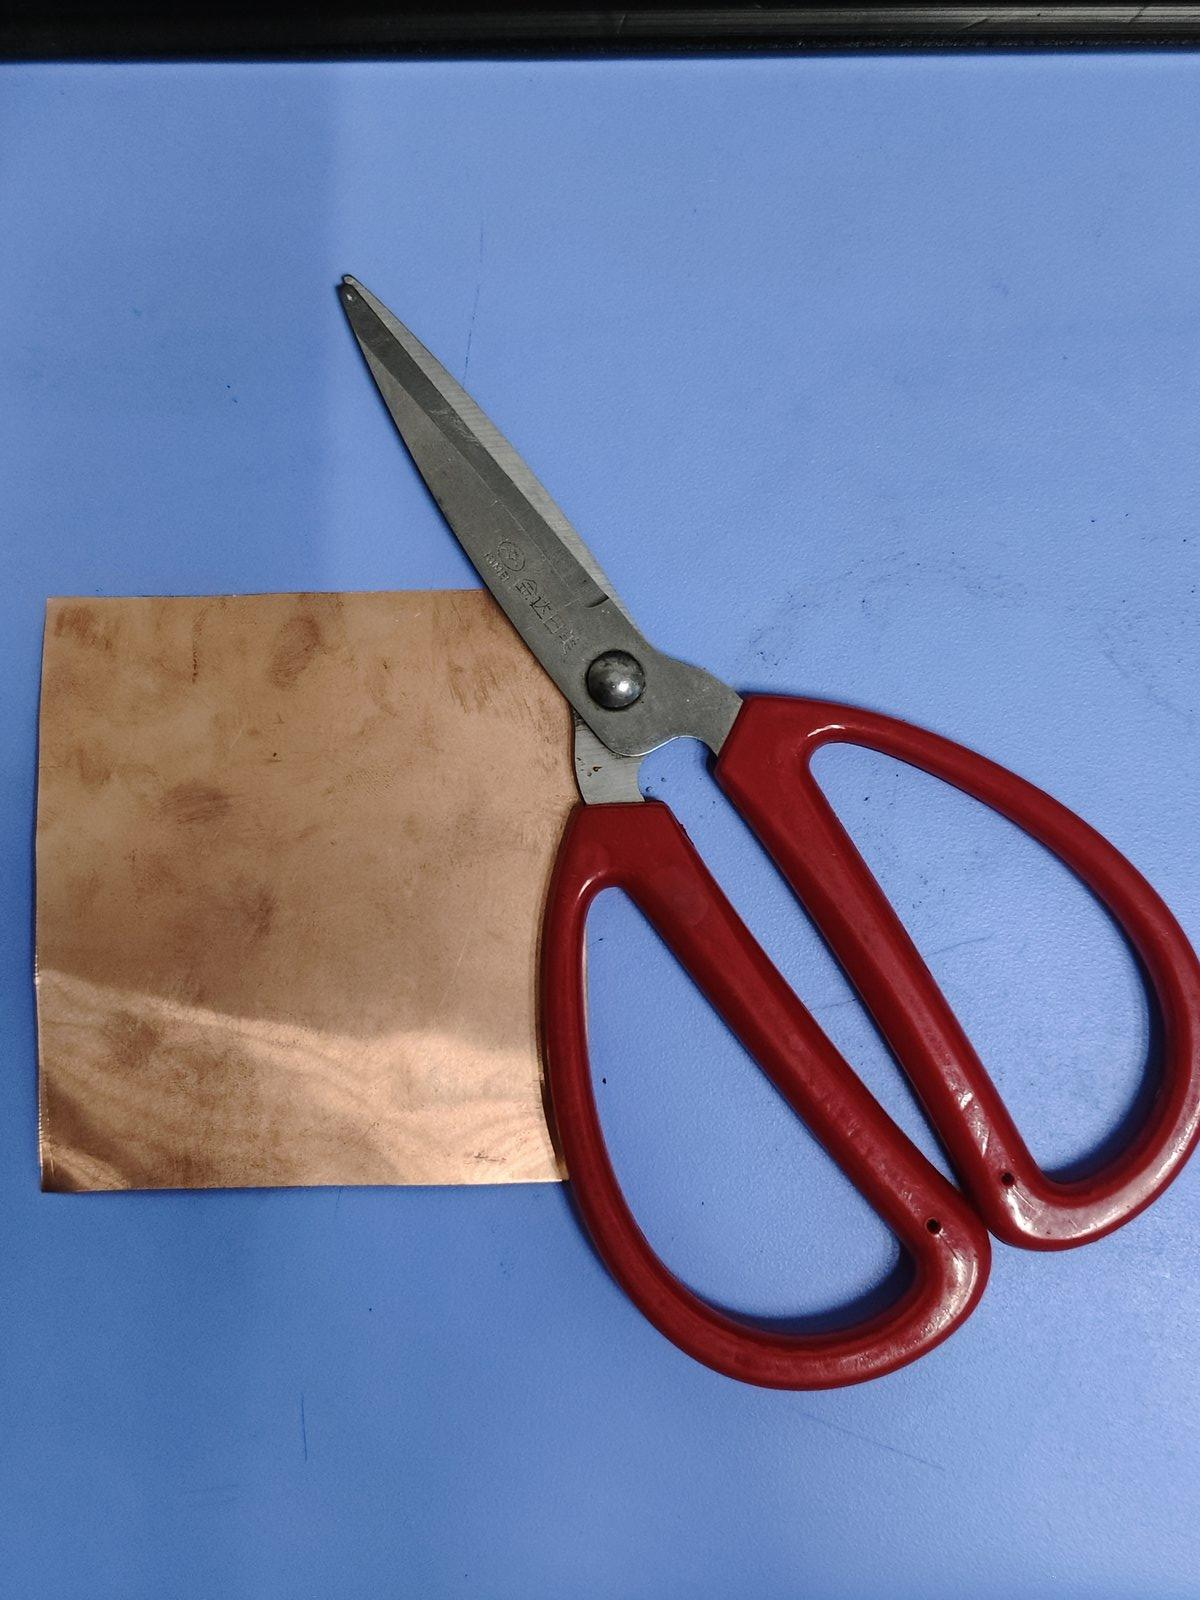
\includegraphics[width=\linewidth]{剪刀与铜片.jpg}
        \caption{剪刀与铜片}
    \end{subfigure}
    \begin{subfigure}{0.22\textwidth}
        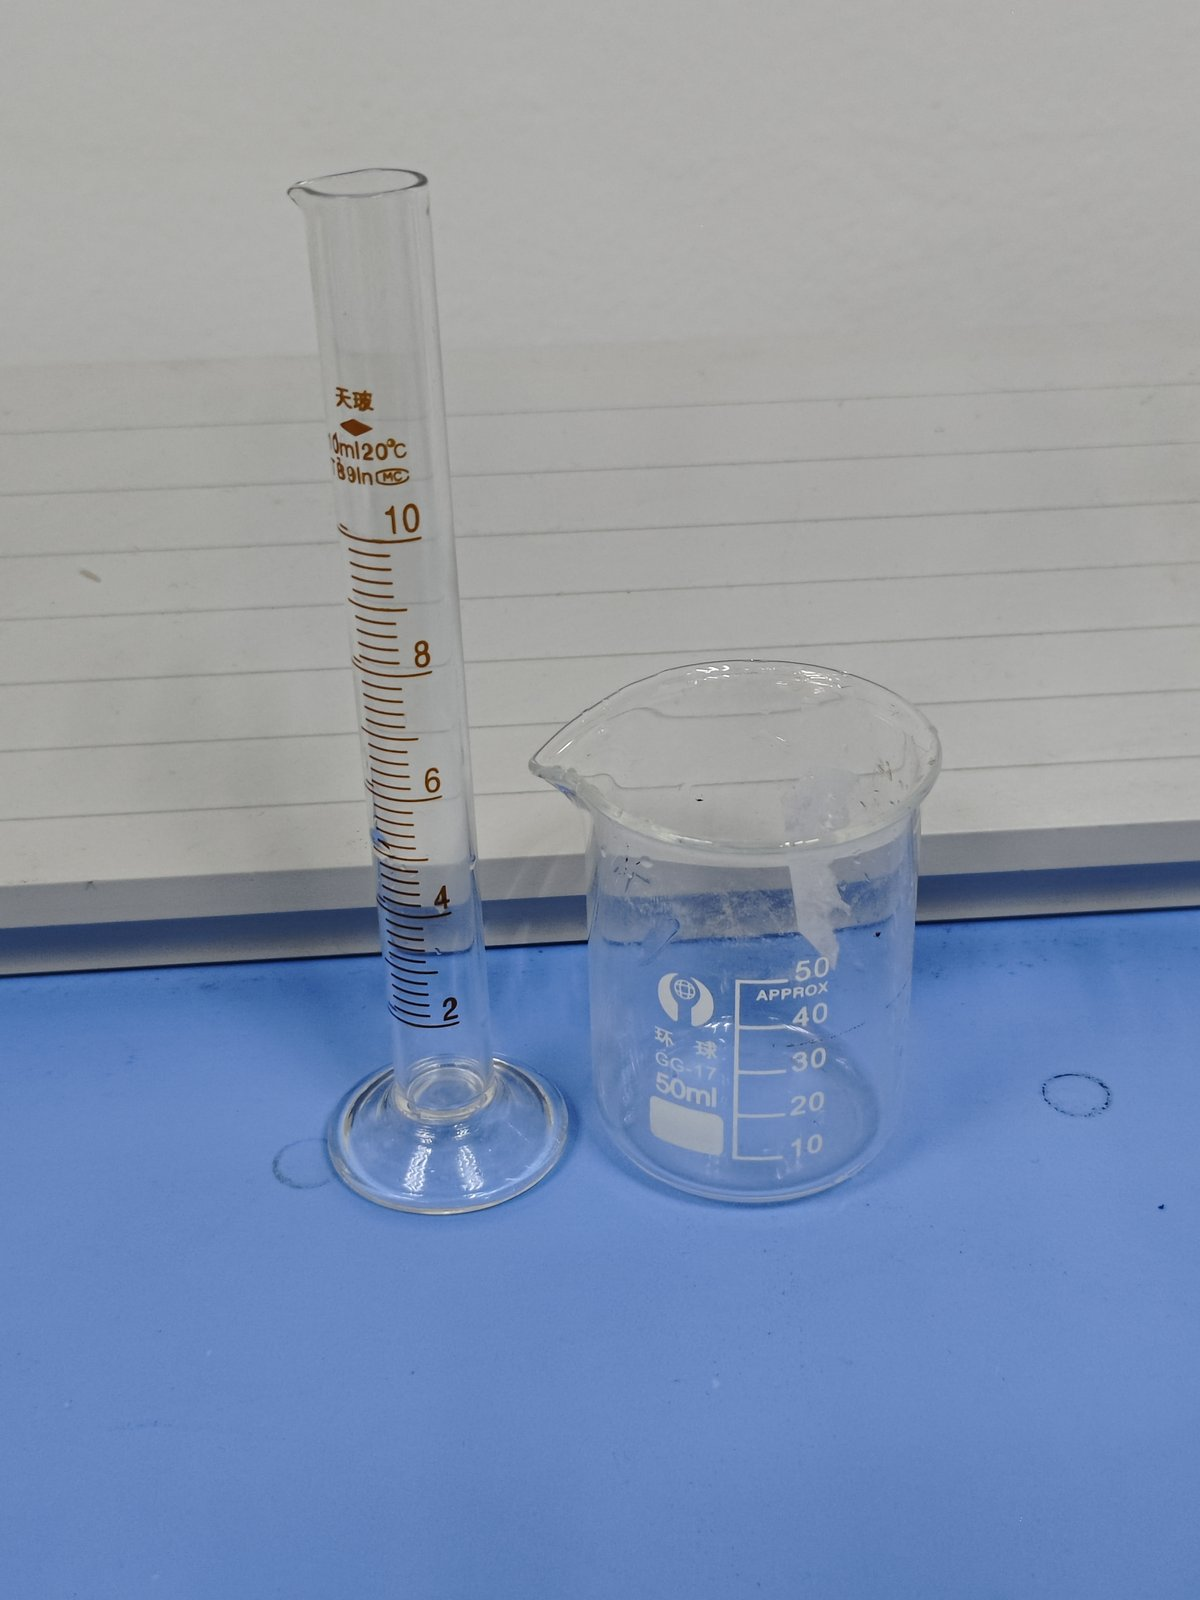
\includegraphics[width=\linewidth]{烧杯与量筒.jpg}
        \caption{烧杯与量筒}
    \end{subfigure}
    \begin{subfigure}{0.22\textwidth}
        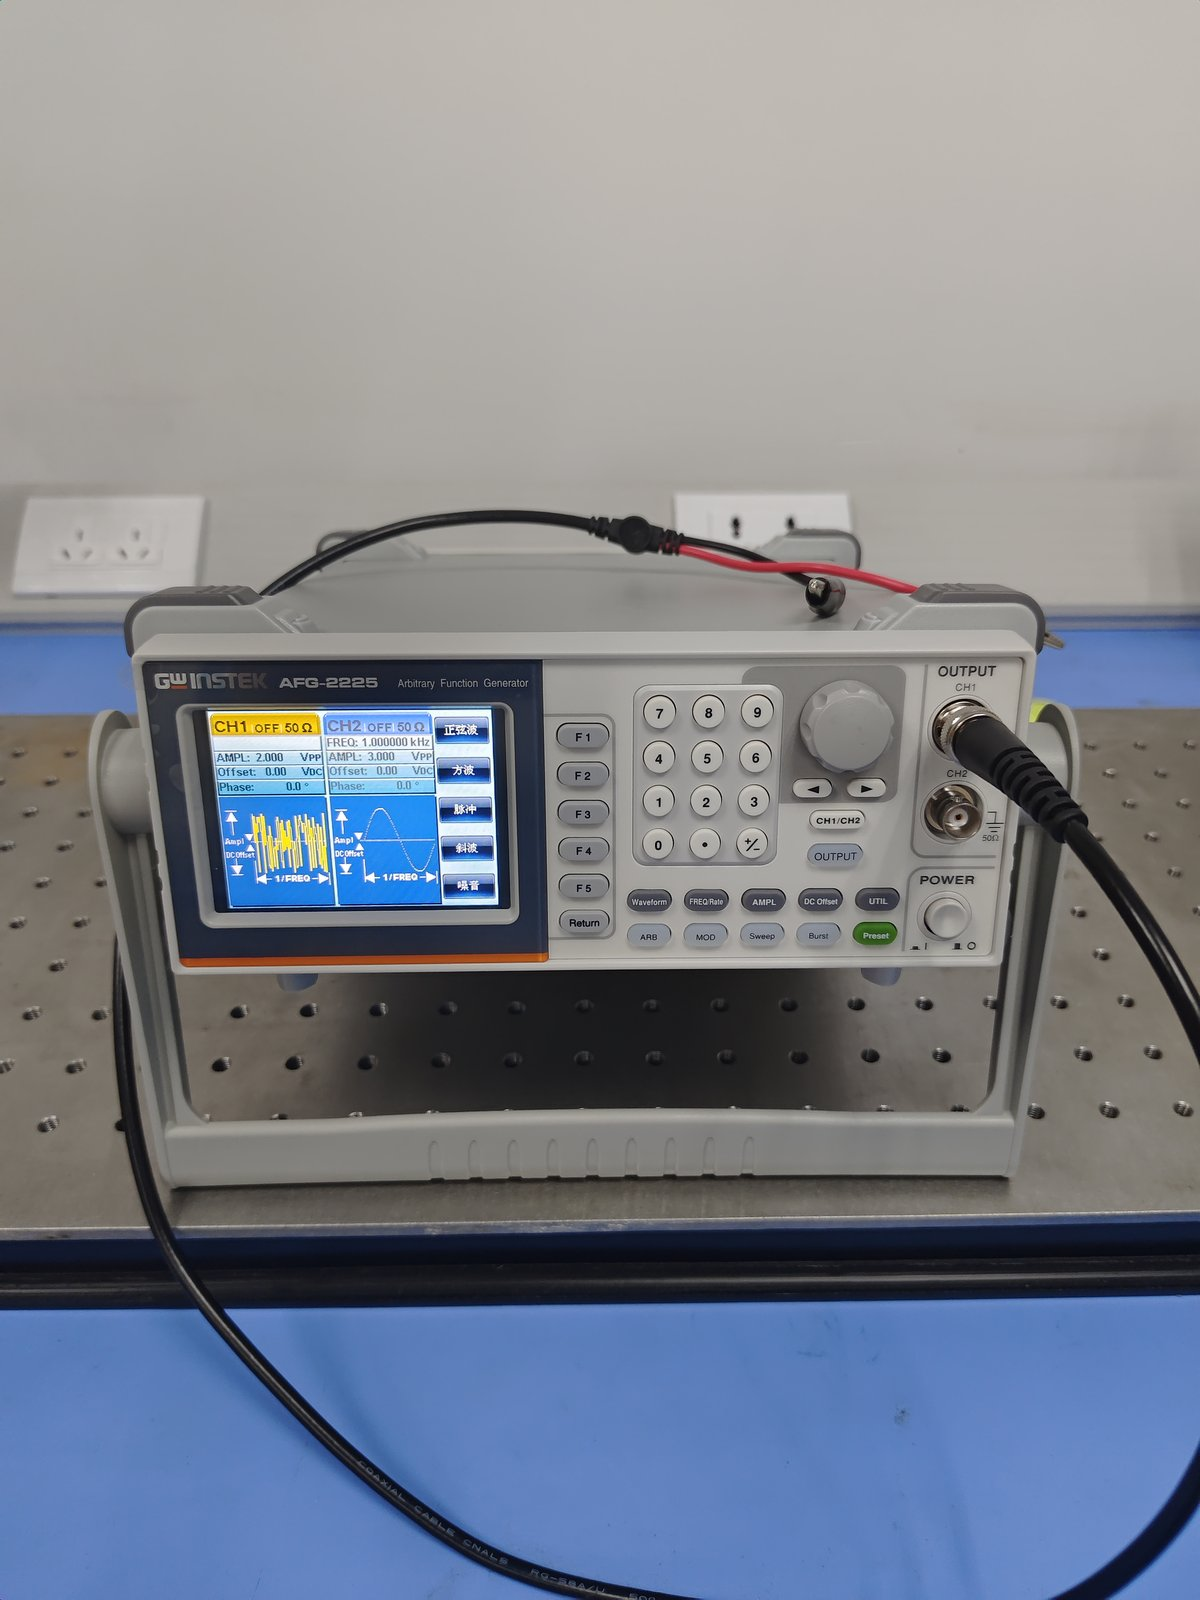
\includegraphics[width=\linewidth]{信号发生器.jpg}
        \caption{信号发生器}
    \end{subfigure}

    \caption{实验仪器}
\end{figure}

\section{实验装置}

\begin{figure}[H]
    \centering
    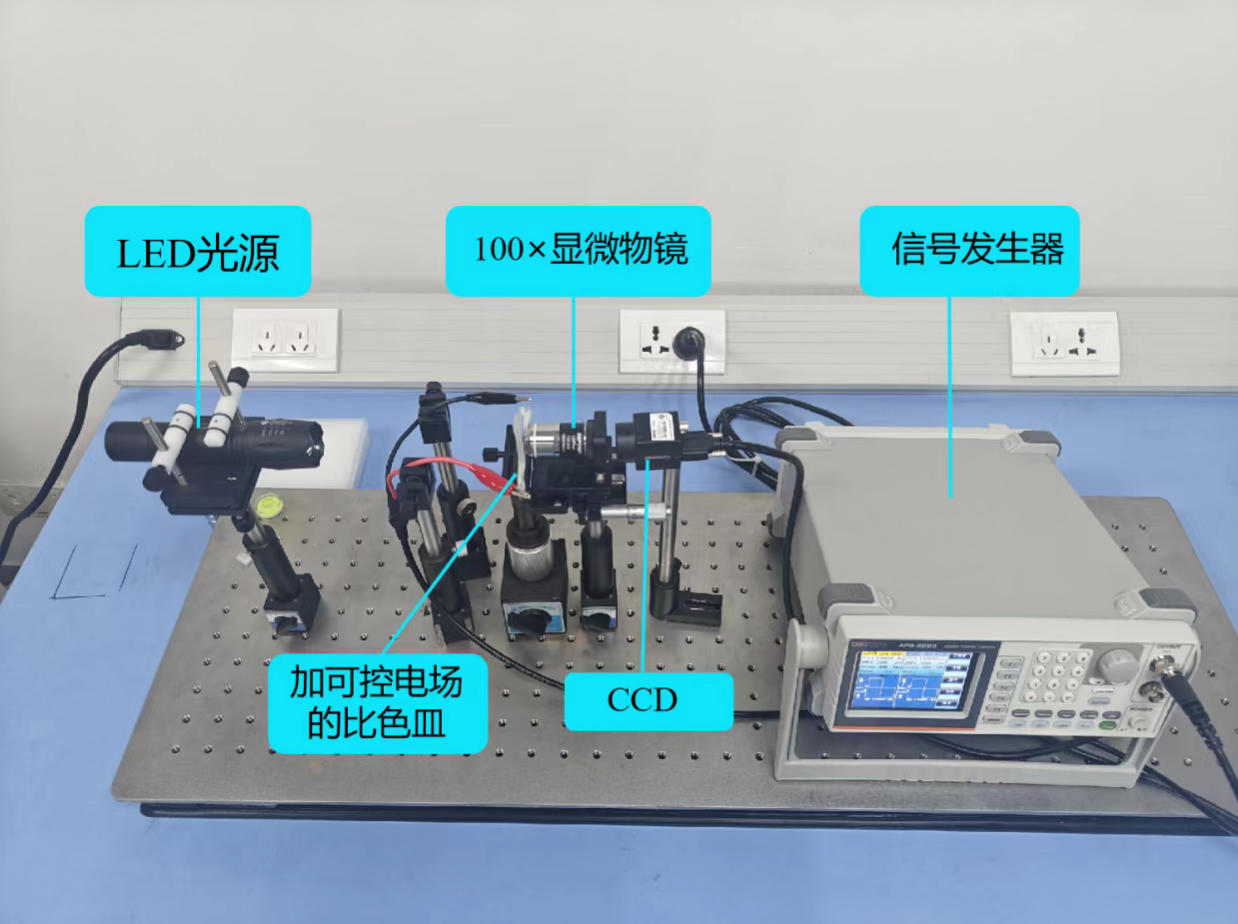
\includegraphics[width=0.9\textwidth]{完整实验装置.jpg}
    \caption{实验装置示意图}
    \label{fig:allsetup}
\end{figure}
\chapter{实验内容}

\section{验证不同粒子直径的小球是布朗运动}
\subsection{实验步骤}
1.按照图~\ref{fig:sets}搭建光路,开启 LED 光源,保证LED光经过聚光镜后均匀照射在比色皿(或分辨率板)上,
固定好LED,显微物镜,和CCD相机后,将分辨率板放在夹具上进行标定实验。
\begin{figure}[H]
    \centering
    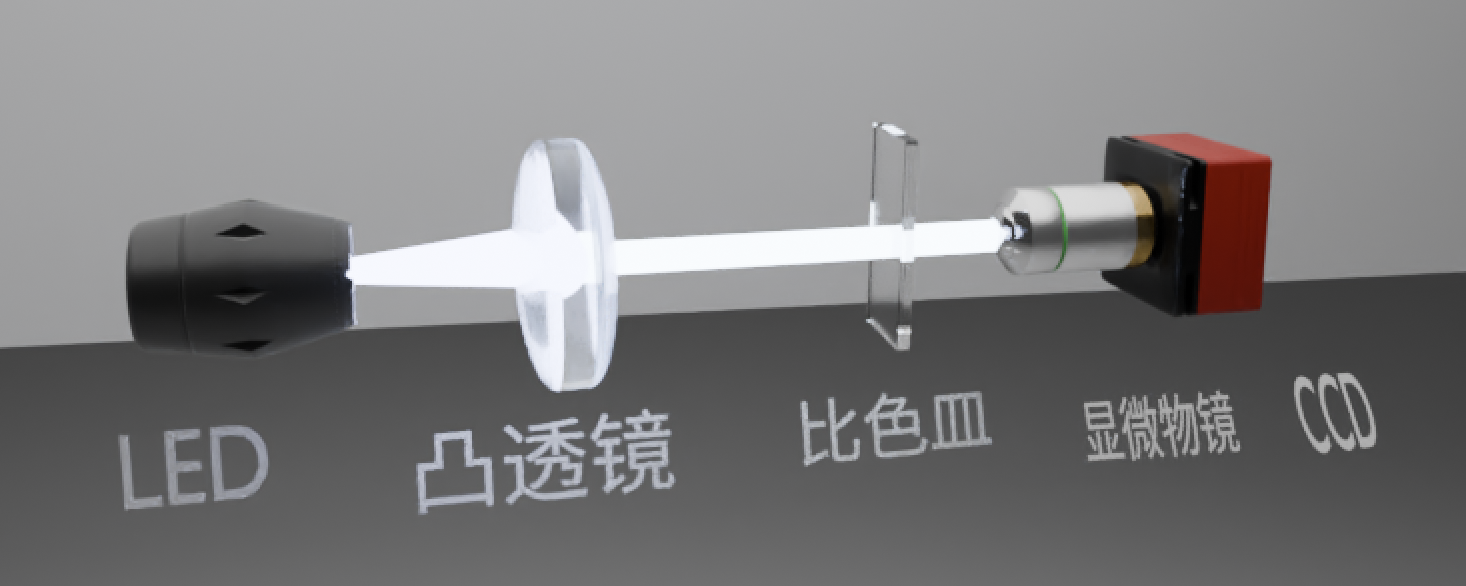
\includegraphics[width=0.9\textwidth]{实验示意图.png}
    \caption{实验装置示意图}
    \label{fig:sets}
\end{figure} 
2.配制适当浓度的不同直径、不同液体粘度的聚苯乙烯(PS)微球。\par
3.将溶液加入比色皿中,放在夹具上静置 0.5--1 h。\par
4.开启 LED,观察 PS 微球,待稳定时收集数据。\par
5.将比色皿取下,拍摄背景图片。\par
6.进行数据处理。\par

\subsection{数据处理}

\section{验证不同噪声强度下的布朗运动}

\section{不同噪声下的布朗运动}
\subsection{实验步骤}
1.使用前面搭建的光路(图~\ref{fig:allsetup}),开启 LED 光源,将分辨率板放在夹具上进行标定。\par
2.配制适当浓度、直径为 500 nm 的聚苯乙烯(PS)微球。\par
3.剪取两片铜片作为电极,使用无水乙醇清洗后晾干。\par
4.将溶液加入比色皿中,放在夹具上,将铜片电极清洗后插入比色皿;连接信号发生器并保证铜片平行紧贴两侧,静置 0.5--1 h。\par
5.开启 LED,观察 PS 微球,待稳定时依次加不同振幅(0--10 V)的电压,收集数据。\par
6.将比色皿取下,拍摄背景图片。\par
7.进行数据处理。\par
\section{熵产生率估算}

\section{注意事项}
(1).每次使用完微量移液器,比色皿和电极片需要用无水乙醇清洗干净,防止污染。\par
(2).实验过程中,尽量避免振动和气流对比色皿的影响。\par
(3).待每次采集微球的运动数据后,需尽快移走比色皿并保持其他部分装置不动和CCD曝光时间相同,尽快拍摄背景图片 \par
\chapter{误差分析}
\chapter{结论与展望}

\chapter{附录}
\section{人员分工}
\renewcommand{\arraystretch}{1.3} % 表格行距调整

\begin{tabularx}{\textwidth}{>{\bfseries}l X}
\toprule
队员 & 分工 \\
\midrule
队员一 & 负责实验数据采集,实验报告的撰写等。 \\
队员二 & 负责热学相关部分原理的推导和微球布朗运动的模拟等。 \\
队员三 & 负责制作ppt和实验采集,查阅文献等。 \\
队员四 & 负责后期数据处理,误差分析,查阅文献等。 \\
\bottomrule
\end{tabularx}


\section{部分代码展示}
\begin{lstlisting}[language=Python, caption=检测微球, label=code:generator]
def filter_stationary_particles(trajectories, max_displacement=2.0, min_frames=10):
    """
    过滤静止不动的粒子(CCD灰尘)
    
    参数:
    trajectories: 轨迹数据
    max_displacement: 最大允许位移(像素),小于此值认为是静止粒子
    min_frames: 最小帧数,少于这个帧数的轨迹直接过滤
    """
    
    filtered_trajectories = []
    stationary_count = 0
    short_trajectory_count = 0
    
    for particle_id, group in trajectories.groupby('particle'):
        # 过滤短轨迹
        if len(group) < min_frames:
            short_trajectory_count += 1
            continue
            
        # 计算粒子的总位移
        start_frame = group['frame'].min()
        end_frame = group['frame'].max()
        
        start_pos = group[group['frame'] == start_frame][['x', 'y']].values[0]
        end_pos = group[group['frame'] == end_frame][['x', 'y']].values[0]
        
        total_displacement = np.sqrt(np.sum((end_pos - start_pos) ** 2))
        
        # 计算RMS位移
        mean_x = group['x'].mean()
        mean_y = group['y'].mean()
        rms_displacement = np.sqrt(np.mean((group['x'] - mean_x) ** 2 + (group['y'] - mean_y) ** 2))
        
        # 过滤静止粒子
        if total_displacement < max_displacement and rms_displacement < max_displacement:
            stationary_count += 1
            continue
        
        # 保留非静止粒子
        filtered_trajectories.append(group)
    
    if filtered_trajectories:
        filtered_df = pd.concat(filtered_trajectories, ignore_index=True)
    else:
        filtered_df = pd.DataFrame(columns=trajectories.columns)
    
    print(f"过滤结果:")
    print(f"  总粒子数: {trajectories['particle'].nunique()}")
    print(f"  静止粒子数: {stationary_count}")
    print(f"  短轨迹粒子数: {short_trajectory_count}")
    print(f"  有效粒子数: {filtered_df['particle'].nunique()}")
    
    return filtered_DataFrame

def batch_detect_particles(frames, params):
    """批量检测所有帧中的粒子"""
    all_features = []
    
    print("开始批量检测粒子...")
    for i, frame in enumerate(frames):
        # 使用trackpy检测粒子
        features = tp.locate(frame, 
                            diameter=params['diameter'],
                            minmass=params['minmass'],
                            separation=params['separation'],
                            noise_size=params['noise_size'],
                            invert=params['invert'])
        
        # 添加帧编号信息
        features['frame'] = i
        all_features.append(features)
        
        if (i + 1) % 50 == 0:
            print(f"已处理 {i + 1}/{len(frames)} 帧,当前帧检测到 {len(features)} 个粒子")
    
    # 合并所有检测结果
    combined_features = pd.concat(all_features, ignore_index=True)
    print(f"\n总共检测到 {len(combined_features)} 个粒子检测结果")
    return combined_features
\end{lstlisting}
首先使用上面的代码进行粒子检测和过滤,得到干净的粒子轨迹数据。然后使用下面的代码进行粒子跟踪、可视化和统计分析。\\
\begin{lstlisting}[language=Python, caption=可视化与计算, label=code:generator]
def track_particles(features_df, search_range=50, memory=5):
    """跟踪粒子运动轨迹"""
    print("开始粒子跟踪...")
    
    # 使用trackpy进行粒子跟踪
    trajectories = tp.link(features_df, 
                          search_range=search_range, 
                          memory=memory,
                          neighbor_strategy='KDTree')
    
    # 计算每个轨迹的粒子数量
    particle_counts = trajectories['particle'].value_counts()
    
    print(f"跟踪完成!")
    print(f"总共跟踪到 {len(particle_counts)} 个独立粒子")
    print(f"轨迹长度统计:")
    print(f"最长轨迹: {particle_counts.max()} 帧")
    print(f"最短轨迹: {particle_counts.min()} 帧")
    print(f"平均轨迹长度: {particle_counts.mean():.2f} 帧")
    
    return trajectories

def visualize_particle_movement(trajectories):
    """可视化粒子运动轨迹"""
    plt.figure(figsize=(12, 10))
    
    # 为每个粒子分配颜色
    particle_ids = trajectories['particle'].unique()
    colors = plt.cm.viridis(np.linspace(0, 1, len(particle_ids)))
    
    for i, particle_id in enumerate(particle_ids):
        group = trajectories[trajectories['particle'] == particle_id]
        if len(group) > 5:  # 只显示有足够数据的轨迹
            plt.plot(group['x'], group['y'], 'o-', 
                    markersize=2, linewidth=1, alpha=0.7, 
                    color=colors[i], label=f'粒子 {particle_id}')
    
    plt.title('粒子运动轨迹', fontsize=16, fontweight='bold')
    plt.xlabel('X坐标 (像素)', fontsize=12)
    plt.ylabel('Y坐标 (像素)', fontsize=12)
    plt.grid(True, alpha=0.3)
    plt.legend(bbox_to_anchor=(1.05, 1), loc='upper left')
    plt.tight_layout()
    plt.show()

def calculate_basic_statistics(trajectories):
    """计算基本统计信息"""
    print("\n轨迹统计信息:")
    print("=" * 40)
    
    # 轨迹长度统计
    trajectory_lengths = trajectories.groupby('particle').size()
    print(f"平均轨迹长度: {trajectory_lengths.mean():.2f} 帧")
    print(f"最长轨迹: {trajectory_lengths.max()} 帧")
    print(f"最短轨迹: {trajectory_lengths.min()} 帧")
    
    # 位移统计
    displacements = []
    for particle_id, group in trajectories.groupby('particle'):
        if len(group) > 1:
            start_pos = group[group['frame'] == group['frame'].min()][['x', 'y']].values[0]
            end_pos = group[group['frame'] == group['frame'].max()][['x', 'y']].values[0]
            displacement = np.sqrt(np.sum((end_pos - start_pos) ** 2))
            displacements.append(displacement)
    
    if displacements:
        print(f"平均位移: {np.mean(displacements):.2f} 像素")
        print(f"最大位移: {np.max(displacements):.2f} 像素")
        print(f"最小位移: {np.min(displacements):.2f} 像素")
    
    print(f"总粒子数: {trajectories['particle'].nunique()}")
    print(f"总数据点: {len(trajectories)}")
\end{lstlisting}

\section{实验数据}

\addcontentsline{toc}{chapter}{参考文献} % 手动加到目录
\bibliographystyle{plain}
\bibliography{refs}
\end{document}
